Informatica → dal francese ``\emph{Informatique}'' = Information +
Automatique

↓

Insieme di tecnologie di tipo elettronico utili per creare,
immagazzinare e elaborare \ul{informazioni}.

↓

Informare vuol dire dare forma a qualcosa, rendere consapevole qualcuno

La minima informazione è il bit (Binary Digit) cioè
l\textquotesingle unità di informazione necessaria per la scelta
effettuata tra due soli eventi ( 0 e 1, vero e falso); in modo da
diminuire l'incertezza.

\paragraph{Sistema informatico VS Sistema
informativo}\label{sistema-informatico-vs-sistema-informativo}

\ul{Sistema informativo}→ Ha lo scopo di produrre ``in tempo utile'',
nelle ``forme appropriate'', ed ai ``giusti livelli'' le sintesi
necessarie per i processi decisionali.

\ul{Sistema informatico} → sottoinsieme del sistema informativo dedicato
alla gestione automatica di informazioni; quindi è l'insieme di parti
con l'obiettivo di archiviare, elaborare e raccogliere informazioni in
maniera elettronica.

\paragraph{Computer}\label{computer}

Il computer è un \emph{elaboratore} \emph{elettronico digitale}:

\begin{itemize}
\item
  \ul{Elaboratore}: macchina in grado di immagazzinare ed elaborare dati
  in base ad una serie di istruzioni;
\item
  \ul{Elettronico}: utilizza componenti elettronici per elaborare le
  informazioni;
\item
  \ul{Digitale}: i dati sono memorizzati mediante cifre binarie;
\end{itemize}

Il calcolatore al suo interno è diviso in:

\begin{itemize}
\item
  \ul{Hardware}: l'insieme di dispositivi (fisici) che compongono il
  calcolatore;
\item
  \ul{Software}: istruzioni e informazioni necessarie per risolvere i
  problemi;
\item
  \ul{Firmware}: è il confine fra le due parti precedenti,
  microprogrammi scritti dai costruttori o memorizzati su speciali
  memorie.
\end{itemize}

\paragraph{Storia del calcolatore}\label{storia-del-calcolatore}

Esistono diverse generazioni di calcolatori, ecco quali:

\begin{enumerate}
\def\labelenumi{\arabic{enumi}.}
\item
  \emph{Gen 0 {[}calcolatori meccanici{]}}: Il primo a costruire
  macchine calcolatrici automatiche fu lo scienziato francese Blaise
  Pascal (Pascalina), un dispositivo a ingranaggi azionati per mezzo di
  una manovella e in grado di effettuare addizioni e sottrazioni;
  aggiornata da Gottfried in modo da fare moltiplicazioni e divisioni.
\item
  \emph{Gen 1 {[}valvole termoioniche e relè{]}}: Massachusetts
  Institute of Technology progettò il Differential Analyzer. Questa
  macchina era in grado di risolvere equazioni differenziali; il primo
  dei calcolatori elettrici e digitali.
\end{enumerate}

\begin{quote}
Alan Mathison Turing riuscì a decrittografare i messaggi tedeschi usando
un calcolatore elettromeccanico che poteva lavorare ad altissima
velocità (Colossus).

Negli anni successivi alla guerra vennero sviluppati gli ENIAC
(Electronic Numerical Integrator And Computer), tra i consulenti c'era
Von Neumann che progettò l'EDVAC composto da registri dentro la CPU
(composta a sua volta da Unità di controllo e aritmetico logica, ALU) e
una memoria principale tutto collegato con bus.

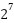
\includegraphics[width=4.28125in,height=2.32292in]{media/image11.png}

Prima di ciò Von Neumann e altri progettarono IAS, denominata macchina
di Von Neumann, una pietra miliare dell'informatica, che influenzò
pesantemente lo sviluppo di tutti i calcolatori successivi.

\textbf{In questa Gen per la priva volta si utilizzano gli 0 e 1
(accesso spento).}
\end{quote}

\begin{enumerate}
\def\labelenumi{\arabic{enumi}.}
\setcounter{enumi}{2}
\item
  \emph{Gen 2 {[}i transistor{]}}: il transistor fu inventato nel 1948
  alla Bell Labs e fruttò ai suoi inventori il premio Nobel per la
  fisica.
\end{enumerate}

\begin{quote}
Primo passo verso la miniaturizzazione che portò alla creazione di
hardware meno ingombranti, più veloci e meno dispendiosi.

Anni `60 la DEC produce il PDP-8 con il BUS.

\textbf{Inizia la miniaturizzazione.}
\end{quote}

\begin{enumerate}
\def\labelenumi{\arabic{enumi}.}
\setcounter{enumi}{3}
\item
  \emph{Gen 3 {[}circuiti integrati{]}}: inventati nel 1958 da Robert
  Noyce permisero di inserire dozzine di transistor su un singolo pezzo
  di silicio e quindi favorirono la costruzione di calcolatori più
  piccoli, più veloci e meno costosi.
\item
  \emph{Gen 4 {[}Very Large Scale Integration{]}}: nel 1971 tre
  ingegneri della Intel crearono il primo microprocessore; comincia così
  l'era dei
\end{enumerate}

\begin{quote}
PC.

Nel 1975 William Gates e Paul Allen, diedero vita a una piccolissima
azienda che elaborava linguaggi per "computer": la Microsoft. Nello
stesso periodo Steve Jobs e Stephen Wozniak costruirono \ul{''Apple
I''}.
\end{quote}

\begin{enumerate}
\def\labelenumi{\arabic{enumi}.}
\setcounter{enumi}{5}
\item
  \emph{Gen 5 {[}Quantistico \& I.A.{]}}: sviluppo dell'hardware
  attraverso i computer quantistici, basati non più sul concetto di bit
  ma di qbit e lo sviluppo del software attraverso l'implementazione
  delle intelligenze artificiali.
\end{enumerate}

\begin{quote}
Nel prossimo futuro i calcolatori saranno sempre più veloci e capaci di
autoprogrammarsi.
\end{quote}

Esiste una ``legge'' che stima come i computer aumentino di potenza ogni
18 mesi, andando a raddoppiare il numero di transistor su un singolo
chip; è la \textbf{legge di Moore}.

\textbf{RAPPRESENTAZIONE DIGITALE DELL'INFORMAZIONE}

L'informazione può essere rappresentata in modo:

\begin{itemize}
\item
  \emph{Digitale}: Ogni dato viene codificato impiegando entità distinte
  individualmente e organizzate in modo opportuno;
\item
  \emph{Analogica}: Basata sull'impiego di dispositivi che realizzano
  una grandezza fisica che può variare in modo continuo.
\end{itemize}

\paragraph{NUMERI A PRECISIONE FINITA}\label{numeri-a-precisione-finita}

Rappresentati con un numero finito di cifre, le operazioni con questi
numeri possono causare i seguenti errori se il loro risultato non
appartiene all'insieme dei valori rappresentabili:

\begin{itemize}
\item
  \emph{Underflow}: il risultato è minore del più piccolo valore
  rappresentabile;
\item
  \emph{Overflow}: il risultato è maggiore del più grande valore
  rappresentabile;
\item
  \emph{Non appartenenza all'insieme}: il risultato non appartiene
  all'insieme dei valori rappresentabili.
\end{itemize}

L'algebra dei numeri a precisione finita è diversa da quella
convenzionale, la proprietà distributiva e la proprietà associativa non
sono rispettate.

\paragraph{NUMERI FLOATING-POINT}\label{numeri-floating-point}

Per il trattamento di valori razionali o reali si adotta una notazione
in cui la gamma dei valori esprimibili è indipendente dal numero di
cifre significative. Questo sistema è detto floating-point. Esprimibile
nel seguente modo:

\begin{quote}
\(n\  = \ f\ *\ 10^{e}\) \({}^{\rightarrow}\)\({}^{esponente}\)
\end{quote}

↓

\emph{mantissa}

La precisione è determinata dalla mantissa \emph{f}, mentre la gamma dei
valori è determinato dall'esponente \emph{e}.

Uno standard permette di valorizzare la mantissa (f) solo in un range
fra 0.1 e 1 (\(0.1 \leq f < 1\)).

\(3.14 = 31.4*10^{- 1}\) \(3.14 = 0.314*10^{1}\)

sbagliato f \textgreater{} 1 corretto \(0.1 \leq f < 1\)

\subparagraph{}\label{section}

\subparagraph{\texorpdfstring{\emph{IEEE
754}}{IEEE 754}}\label{ieee-754}

Con l'introduzione del seguente standard si sono uniti tutti i
calcolatori su un unico formato per i floating-point binari. Ne esistono
3 formati:

\begin{enumerate}
\def\labelenumi{\arabic{enumi}.}
\item
  \emph{Singola precisione}: Totale 32 bit {[}1 per il segno, 8 per gli
  esponenti, 23 mantissa{]};
\item
  \emph{Doppia precisione}: Totale 64 bit {[}1 per il segno, 11 per gli
  esponenti, 52 mantissa{]};
\item
  \emph{Precisione estesa};
\end{enumerate}

Per calcolare l'eccesso si usa la formula \(2^{(n - 1)} - 1\), con n =
numero di bit.

Per calcolare in numero decimale avente il numero binario floating point
si fa così:

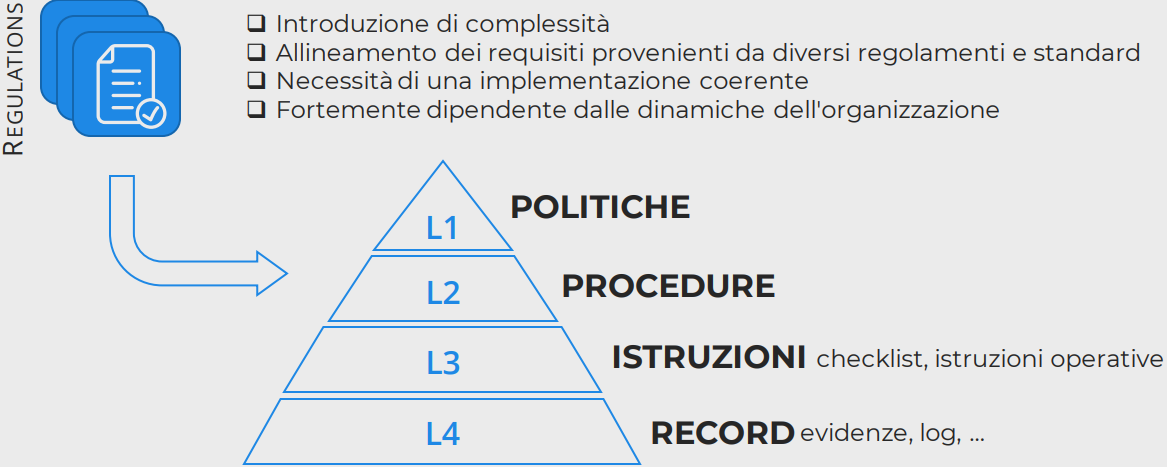
\includegraphics[width=6.26772in,height=2.59722in]{media/image18.png}

\subparagraph{}\label{section-1}

\subparagraph{}\label{section-2}

\subparagraph{Es:}\label{es}

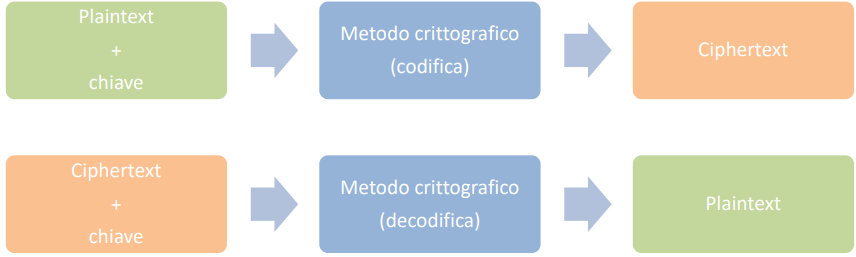
\includegraphics[width=6.26772in,height=2.88889in]{media/image19.png}

\subparagraph{\texorpdfstring{\emph{Normalizzazione}}{Normalizzazione}}\label{normalizzazione}

La mantissa binaria normalizzata deve presentare un 1 a sinistra della
virgola binaria. L'esponente deve essere aggiustato di conseguenza.

Esempio di normalizzazione:

\({4568.1875}_{10}\)

\textbf{cambiamo la base}

1000111011000.0011

\textbf{normalizzo spostando la virgola di tot posizioni in modo da
avere un 1. davanti}

1.0001110110000011 * \(2^{12}\) {[}12 sono le pos. spostate{]}

\textbf{esprimo l'esponente in eccesso (127)}

12 + 127 = 139 → 10001011 \emph{{[}il 127 è dato da} \(2{}^{n - 1} - 1\)
\emph{dove n = num. bit esponente{]}}

\textbf{rappresento il tutto in modo corretto}

0 1 0 0 0 1 0 1 1 0 0 0 1 1 1 0 1 1 0 0 0 0 0 1 1 0 0 0 0 0 0 0

↓ ↓ ↓

segno esponente mantissa normalizzata

\paragraph{SISTEMI DI NUMERAZIONE
INFORMATICA}\label{sistemi-di-numerazione-informatica}

I sistemi di numerazione più utilizzati in informatica:

\begin{itemize}
\item
  Sistema decimale (base=10) 0 1 2 3 4 5 6 7 8 9 ;
\item
  Sistema binario (base=2) 0 1: ogni cifra, detta bit (Binary digIT),
  può essere rappresentata direttamente tramite un livello elettrico di
  tensione ;
\item
  Sistema ottale (base=8) 0 1 2 3 4 5 6 7;
\item
  Sistema esadecimale (base=16) 0 1 2 3 4 5 6 7 8 9 A B C D E F: è
  utilizzato poiché è molto compatto e ben si presta alla traduzione in
  valori binari, poiché ogni cifra corrisponde esattamente a 4 cifre
  binarie.
\end{itemize}

Tutti questi sistemi sono a notazione posizionale, i sistemi di
numerazione posizionale associano alle cifre un diverso valore in base
alla posizione che occupano nella stringa che compone il numero.

\paragraph{CONVERSIONI TRA BASI}\label{conversioni-tra-basi}

Tabella utile per le conversioni:

\begin{longtable}[]{@{}
  >{\raggedright\arraybackslash}p{(\linewidth - 2\tabcolsep) * \real{0.4659}}
  >{\raggedright\arraybackslash}p{(\linewidth - 2\tabcolsep) * \real{0.5341}}@{}}
\toprule\noalign{}
\begin{minipage}[b]{\linewidth}\centering
BINARIO
\end{minipage} & \begin{minipage}[b]{\linewidth}\centering
OTTALE/ESADECIMALE
\end{minipage} \\
\begin{minipage}[b]{\linewidth}\centering
0000
\end{minipage} & \begin{minipage}[b]{\linewidth}\centering
0
\end{minipage} \\
\begin{minipage}[b]{\linewidth}\centering
0001
\end{minipage} & \begin{minipage}[b]{\linewidth}\centering
1
\end{minipage} \\
\begin{minipage}[b]{\linewidth}\centering
0010
\end{minipage} & \begin{minipage}[b]{\linewidth}\centering
2
\end{minipage} \\
\begin{minipage}[b]{\linewidth}\centering
0011
\end{minipage} & \begin{minipage}[b]{\linewidth}\centering
3
\end{minipage} \\
\begin{minipage}[b]{\linewidth}\centering
0100
\end{minipage} & \begin{minipage}[b]{\linewidth}\centering
4
\end{minipage} \\
\begin{minipage}[b]{\linewidth}\centering
0101
\end{minipage} & \begin{minipage}[b]{\linewidth}\centering
5
\end{minipage} \\
\begin{minipage}[b]{\linewidth}\centering
0110
\end{minipage} & \begin{minipage}[b]{\linewidth}\centering
6
\end{minipage} \\
\begin{minipage}[b]{\linewidth}\centering
0111
\end{minipage} & \begin{minipage}[b]{\linewidth}\centering
7
\end{minipage} \\
\begin{minipage}[b]{\linewidth}\centering
1000
\end{minipage} & \begin{minipage}[b]{\linewidth}\centering
8
\end{minipage} \\
\begin{minipage}[b]{\linewidth}\centering
1001
\end{minipage} & \begin{minipage}[b]{\linewidth}\centering
9
\end{minipage} \\
\begin{minipage}[b]{\linewidth}\centering
1010
\end{minipage} & \begin{minipage}[b]{\linewidth}\centering
A
\end{minipage} \\
\begin{minipage}[b]{\linewidth}\centering
1011
\end{minipage} & \begin{minipage}[b]{\linewidth}\centering
B
\end{minipage} \\
\begin{minipage}[b]{\linewidth}\centering
1100
\end{minipage} & \begin{minipage}[b]{\linewidth}\centering
C
\end{minipage} \\
\begin{minipage}[b]{\linewidth}\centering
1101
\end{minipage} & \begin{minipage}[b]{\linewidth}\centering
D
\end{minipage} \\
\begin{minipage}[b]{\linewidth}\centering
1110
\end{minipage} & \begin{minipage}[b]{\linewidth}\centering
E
\end{minipage} \\
\begin{minipage}[b]{\linewidth}\centering
1111
\end{minipage} & \begin{minipage}[b]{\linewidth}\centering
F
\end{minipage} \\
\midrule\noalign{}
\endhead
\bottomrule\noalign{}
\endlastfoot
\end{longtable}

\subparagraph{\texorpdfstring{\emph{Binario →
Decimale}}{Binario → Decimale}}\label{binario-decimale}

Per convertire qualsiasi numero binario in uno decimale basta
moltiplicare il numero per la base elevata alla posizione.

Es: 1 0 0 1 1 0 0 1

7 6 5 4 3 2 1 0

1*\(2^{7}\) + 1*\(2^{4}\ \) + 1*\(2^{3}\) + 1*\(2^{0}\) = 128 + 16 + 8 +
1 = 15310

Per convertire una parte frazionaria (Es: 0.101) usiamo lo stesso
ragionamento ma con i numeri ad esponente negativo:

Es: 0.1 0 1

-1 -2 -3

1*\(2^{- 1}\) + 0*\(2^{- 2}\ \) + 1*\(2^{- 3}\) = 0,5 + 0 + 0,125 =
0,62510

\subparagraph{\texorpdfstring{\emph{Ottale →
Decimale}}{Ottale → Decimale}}\label{ottale-decimale}

Come prima prendiamo il numero e moltiplichiamo ogni cifra per la base
elevata alla posizione:

Es: \(32_{8}\) → 3*\(8^{1}\) + 2*\(8^{0}\) = 24 + 2 = \(26_{10}\)

\subparagraph{\texorpdfstring{\emph{Esadecimale →
Decimale}}{Esadecimale → Decimale}}\label{esadecimale-decimale}

Come prima prendiamo il numero e moltiplichiamo ogni cifra per la base
elevata alla posizione, in questo caso le cifre numeriche si fermano al
9, dal 10 al 15 le cifre diventano lettere (dalla A alla F):

Es: 1\(A_{16}\) → \(1*16^{1}\) + \(10*16^{0}\) = 16 + 10 = \(26_{10}\)

\subparagraph{\texorpdfstring{\emph{Binario →
Ottale}}{Binario → Ottale}}\label{binario-ottale}

Convertiamo le cifre binarie a gruppi di 3:

Es. 1 0 1 1 1 1 0 → ( 001) (011) (110)

↓ ↓ ↓

1 3 6 = \(136_{8}\)

\subparagraph{\texorpdfstring{\emph{Ottale → Binario}
}{Ottale → Binario }}\label{ottale-binario}

Procedimento inverso rispetto al precedente:

Es: \(136_{8}\) = ( 001) (011) (110) → 1 0 1 1 1 1 0

\subparagraph{}\label{section-3}

\subparagraph{\texorpdfstring{\emph{Esadecimale → Binario}
}{Esadecimale → Binario }}\label{esadecimale-binario}

Convertiamo le cifre esadecimali a gruppi di 4:

Es: \({7BA3}_{16}\) = (0111) (1011) (1010) (0011)

↓ ↓ ↓ ↓

7 B A 3

\subparagraph{\texorpdfstring{\emph{Decimale → Binario}
}{Decimale → Binario }}\label{decimale-binario}

Esistono due metodi per convertire da base 10 a base 2, ecco quali:

\begin{itemize}
\item
  Metodo 1 {[}Generale{]}:
\end{itemize}

\begin{quote}
Si procede sottraendo la più grande potenza di 2 abbastanza grande da
contenere il numero da convertire, andando poi a mettere 1 nelle
posizioni dell'esponente.

Per rendere più veloce il procedimento possiamo fare somme con i
risultati delle potenze di 2, Es:

138 = 128 + 8 + 2

↓ ↓ ↓
\end{quote}

\(2^{7}\) \({2^{3}}_{}\) \({2^{1}}_{}\) = 10001010

\begin{itemize}
\item
  Metodo 2 {[}Divisione{]}:
\end{itemize}

\begin{quote}
In questo metodo andiamo a dividere per 2 il numero e contando se il
resto è 0 o 1, alla fine delle divisioni prendiamo i resti in modo
ricorsivo. Es:

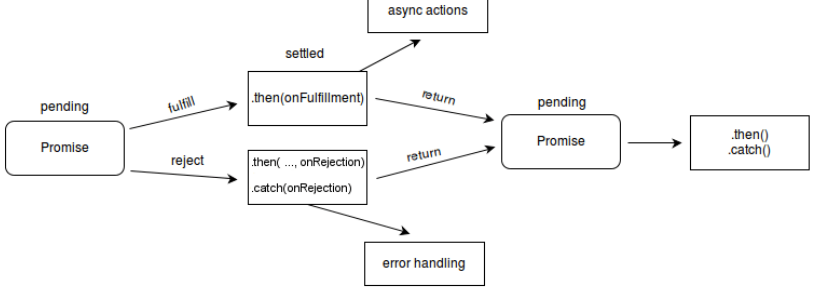
\includegraphics[width=4.02083in,height=5.0625in]{media/image7.png}\(\)
\end{quote}

\begin{itemize}
\item
  Conversione parte frazionaria:
\end{itemize}

\begin{quote}
Per convertire la parte a destra della virgola in un numero binario,
dopo aver convertito normalmente la parte intera, dobbiamo moltiplicare
la parte frazionaria per 2, se il risultato è \textgreater{} di 1 allora
sottraiamo 1 per poi andare a moltiplicare di nuovo e ripetere i
passaggi fino a quando non otteniamo come risultato 1 oppure un
risultato già ottenuto. Esempio:

0,6

↓

0,6 * 2 = 1,2 (\textgreater1)

↓

1,2 -1 = 0,2

↓

0,2 * 2 = 0,4 (\textless1 niente sottrazione)

↓

0,4 * 2 = 0,8 (\textless1 niente sottrazione)

↓

0,8 * 2 = 1,6 (\textgreater1)

↓

1,6 - 1 = 0,6 (risultato già ottenuto, finiamo qui)

Ora per prendere il numero binario andiamo semplicemente a prendere i
numeri prima della virgola nei risultati \textbf{in maniera non
ricorsiva} !!!

Quindi il risultato sarà:

0,6 = 0.1001

\emph{(non prendo i risultati delle sottrazioni)}
\end{quote}

\paragraph{ARITMETICA DEL CALCOLATORE}\label{aritmetica-del-calcolatore}

Diversa da quella comunemente utilizzata dalle persone; la precisione
con cui i numeri possono essere espressi è finita.

Per rappresentare i numeri si utilizza il sistema binario.

La più importante unità di misura dell'informazione manipolata dal
calcolatore è il BYTE, composto da 8 bit; sequenze di bit più lunghe di
un byte sono denominate WORD.

\subparagraph{\texorpdfstring{\emph{Somma}}{Somma}}\label{somma}

Il procedimento di somma binaria è equivalente a quello nel sistema
decimale con eccezione del riporto che si genera quando entrambi gli
addendi hanno valore 1. Es:

0 0 1 1 +

0 1 0 1 =

━━━━━

0 1 1 0 \emph{risultato}

0 0 0 1 \emph{riporto}

\begin{itemize}
\item
  La somma è uguale a 1 solo se la coppia di cifre è diversa.
\item
  Il riporto è uguale a 1 solo se entrambe le cifre sono uno.
\item
  In tutti gli altri casi produce 0.
\end{itemize}

\emph{L'ultimo riporto viene messo nel risultato}

\subparagraph{\texorpdfstring{\emph{Numeri binari
negativi}}{Numeri binari negativi}}\label{numeri-binari-negativi}

Prima di vedere la sottrazione bisogna saper negare un numero, esistono
4 metodi:

\begin{enumerate}
\def\labelenumi{\arabic{enumi}.}
\item
  \emph{Grandezza a segno}: prevede l'utilizzo del bit più a sinistra
  per indicare il segno: 0 il +, 1 il -.
\end{enumerate}

\begin{quote}
Es:

76 ➔ 01001100 -76 ➔ 11001100
\end{quote}

\begin{enumerate}
\def\labelenumi{\arabic{enumi}.}
\setcounter{enumi}{1}
\item
  \emph{Complemento a uno}: andiamo a negare il numero, invertendo lo 0
  con l'1 e viceversa.
\end{enumerate}

\begin{quote}
Es:

-(76) ➔ -(01001100) ➔ 10110011
\end{quote}

\begin{enumerate}
\def\labelenumi{\arabic{enumi}.}
\setcounter{enumi}{2}
\item
  \emph{Complemento a due}: prendiamo il numero negato e aggiungiamo 1.
\end{enumerate}

\begin{quote}
Es:

-(76) ➔ -(01001100) ➔ 10110011 ➔ 10110100
\end{quote}

\begin{enumerate}
\def\labelenumi{\arabic{enumi}.}
\setcounter{enumi}{3}
\item
  \emph{Eccesso} \(2^{m - 1}\): Rappresenta i numeri come somma di se
  stessi con 2m-1 dove m è il numero di bit utilizzati per rappresentare
  il valore.
\end{enumerate}

\begin{quote}
Es {[}con m=8 quindi il num. è memorizzato in un byte{]}:

\(2^{m - 1} = 2^{7} = 128\) / -76 ➔ -76+128 = 52 = 00110100
\end{quote}

\subparagraph{\texorpdfstring{\emph{Sottrazione}}{Sottrazione}}\label{sottrazione}

Con i numeri binari si preferisce sommare un numero positivo ad uno
negativo piuttosto che fare una sottrazione.

Si parla quindi di \emph{somma tra numeri binari in complemento a due},
andando a utilizzare questo metodo:

\begin{itemize}
\item
  Il riporto generato dai bit più a sinistra viene ignorato.
\item
  Se gli addendi sono di segno opposto non si può verificare un
  overflow.
\item
  L'overflow si verifica se il riporto generato nel sommare i bit di
  segno è diverso dal riporto utilizzato per sommare i bit di segno.
\end{itemize}

Es:

Addendo 10 0 0 0 0 1 0 1 0

Addendo -3 1 1 1 1 1 1 0 1

━━━━━━━━━━━━━━━

Somma 7 0 0 0 0 0 1 1 1

Riporti 1 1 1 1 1 0 0 0

↓

riporto ignorato

\subparagraph{\texorpdfstring{\emph{Prodotto}}{Prodotto}}\label{prodotto}

Il procedimento del prodotto viene riportato all'addizione in questo
modo:

\begin{itemize}
\item
  Ogni cifra 1 del moltiplicatore fa scorrere a sinistra le cifre del
  moltiplicando, aggiungendo tanti 0 quanti ne richiede la sua
  posizione.
\item
  I numeri così ottenuti vengono memorizzati e sommati tra di loro.
\end{itemize}

Es: 3 2 1 ← posizioni

70*14 = 01000110 * 0000\hl{111}0

↓

dovrò sommare il 70

per se stesso 3 volte (num di 1 = 3) e

ogni volta aggiungere tanti 0 in base alla posizione degli 1

1 0 0 0 1 1 0 0 +

1 0 0 0 1 1 0 0 0 =

━━━━━━━━━

1 1 0 1 0 0 1 0 0 +

1 0 0 0 1 1 0 0 0 0 =

━━━━━━━━━

1 1 1 1 0 1 0 1 0 0 = \(980_{10}\)

\textbf{CODIFICA DELL'INFORMAZIONE}

\paragraph{CODIFICA DEI CARATTERI}\label{codifica-dei-caratteri}

Ogni calcolatore dispone di un set di caratteri codificati sotto forma
di numeri. La mappatura di essi è detta ``tabella dei caratteri''.

\subparagraph{\texorpdfstring{\emph{ASCII}}{ASCII}}\label{ascii}

Utilizza 7 bit (l'8° usato per il controllo) con 128 combinazioni. I
caratteri da 0 a 1F sono detti di controllo, non vengono stampati.

All'ASCII sono state aggiunte diverse estensioni per aggiungere
caratteri non rappresentabili in precedenza, come ad esempio il
\emph{Latin-1} con 8 bit con l'aggiunta delle lettere latine, accenti,
ecc.

\subparagraph{\texorpdfstring{\emph{UNICODE}}{UNICODE}}\label{unicode}

Visto che l'ASCII non poteva rappresentare tutti i caratteri dei vari
alfabeti si è scelto di creare un unico set per tutto il mondo,
l'\emph{Unicode} con 2 byte (16 bit) quindi da 0 65000 circa
combinazioni.

\subparagraph{\texorpdfstring{\emph{UTF-8}}{UTF-8}}\label{utf-8}

il Consorzio UNICODE ha sviluppato lo standard UTF-8 che prevede una
rappresentazione dinamica dei caratteri da 1 a 4 byte per risolvere i
problemi di compatibilità online fra mittente e destinatario.

\paragraph{CODIFICA DELLE IMMAGINI}\label{codifica-delle-immagini}

Le immagini si dividono in rester (scalari) e vettoriali (geometriche).

\subparagraph{\texorpdfstring{\emph{Raster}}{Raster}}\label{raster}

In questa tipologia l'immagine è un insieme di parti distinte che
possono essere codificate separatamente con sequenze di bit. Queste
parti vanno discretizzate (scomposizione dell'immagine in un reticolo di
punti) e quantizzate (codifica di ogni pixel con una sequenza di bit).

L'immagine è un insieme di pixel dove ognuno rappresenta un colore che
insieme ad altri vanno a formare un'immagine.

La discretizzazione prevede:

\begin{itemize}
\item
  \emph{Definizione}: DPI (dot per inches) cioè il numero di pixel;
\item
  \emph{Risoluzione}: dimensione griglia.
\end{itemize}

La Quantizzazione prevede la rappresentazione di ogni pixel con una
sequenza di bit, tale rappresentazione è nota come codifica bitmap.

\subparagraph{\texorpdfstring{\emph{Vettoriali}}{Vettoriali}}\label{vettoriali}

Si affidano a equazioni matematiche per disegnare le immagini, per
questo è flessibile, le immagini possono essere ingrandite o
rimpicciolite senza compromettere la qualità.

Si possono convertire in jpg e png ma non viceversa.

\subparagraph{\texorpdfstring{\emph{Compressione}}{Compressione}}\label{compressione}

Per risparmiare sulla dimensione si:

\begin{itemize}
\item
  usa una tavolozza (palette) per contenere i sottoinsiemi di colori
  rappresentabili;
\item
  usano tecniche (\emph{TIFF}) di compressione cercando di raggruppare
  le aree che hanno caratteristiche comuni;
\item
  usano tecniche (\emph{GIF, JPG}) di compressione che sfruttano la
  caratteristica dell'occhio umano di essere poco sensibile a lievi
  cambiamenti di colore in punti contigui, e quindi eliminano questi
  lievi cambiamenti appiattendo il colore dell'immagine.
\end{itemize}

\paragraph{CODIFICA DEI SUONI}\label{codifica-dei-suoni}

Per rappresentare le onde sonore che rappresentano il suono si usa la
quantizzazione e il campionamento:

\begin{itemize}
\item
  \emph{campionamento}: scelta di istanti in cui considerare il valore
  del segnale;
\item
  \emph{quantizzazione}: codifica dei campioni con un numero predefinito
  di bit.
\end{itemize}

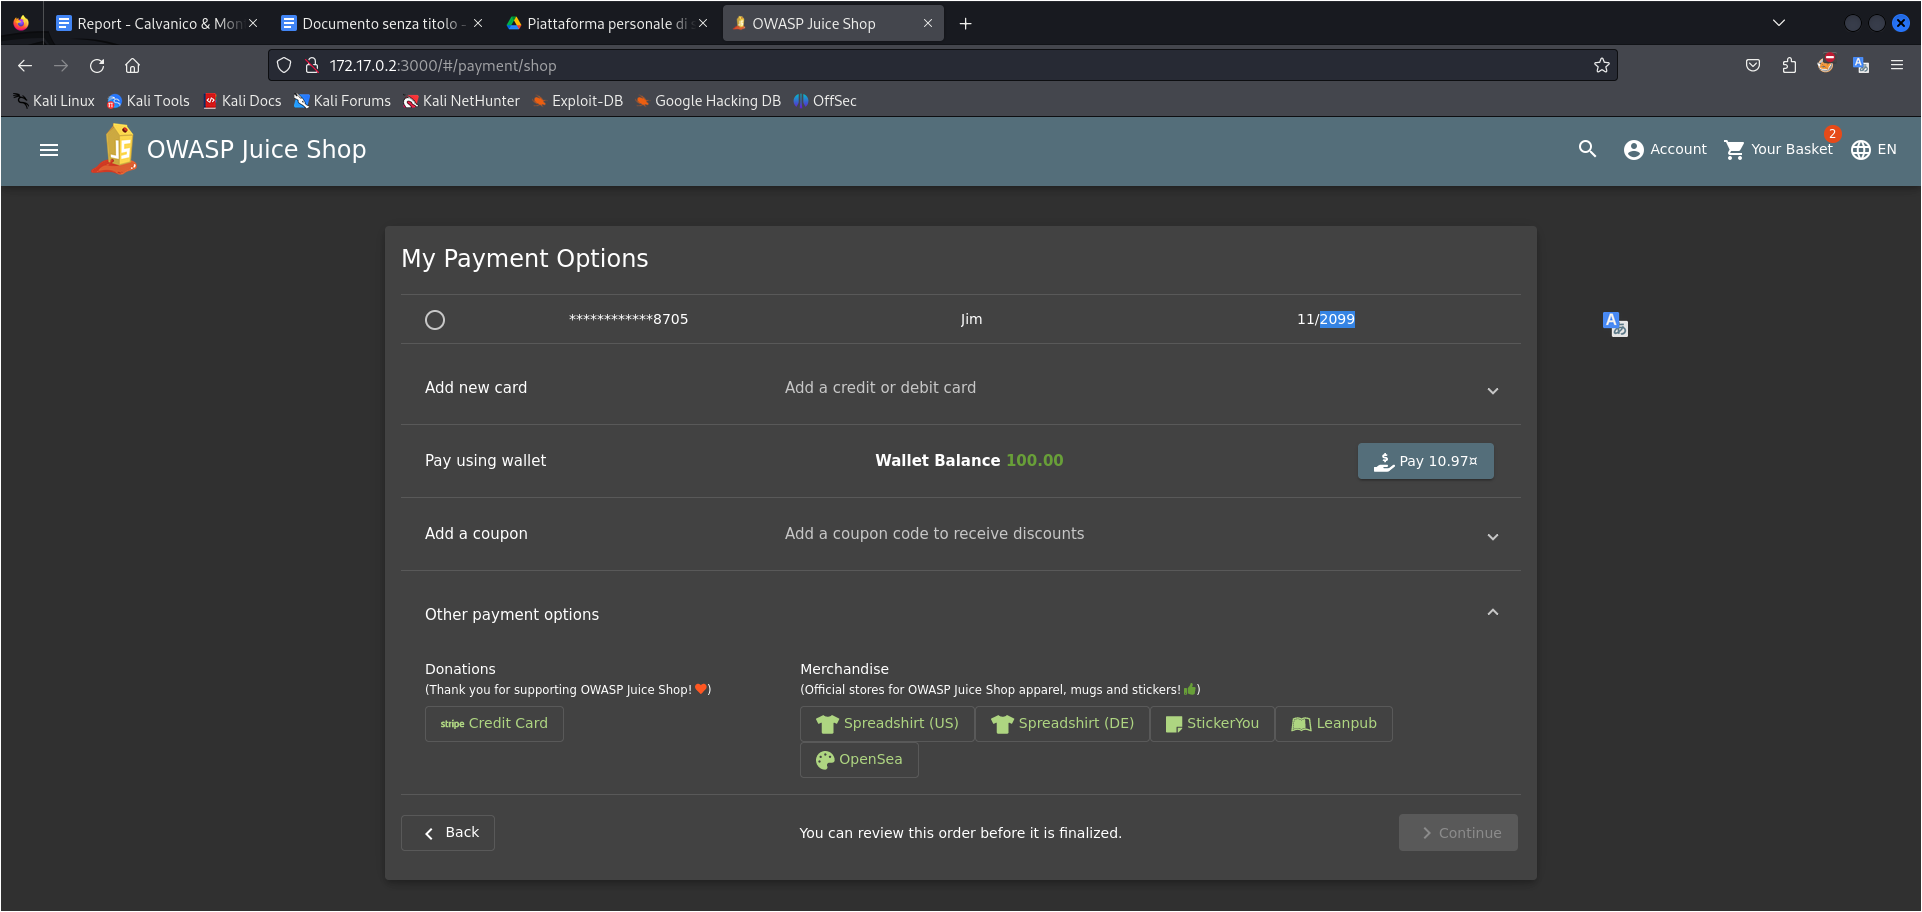
\includegraphics[width=6.21354in,height=2.11458in]{media/image12.png}

Questo è il suono in maniera analogica.

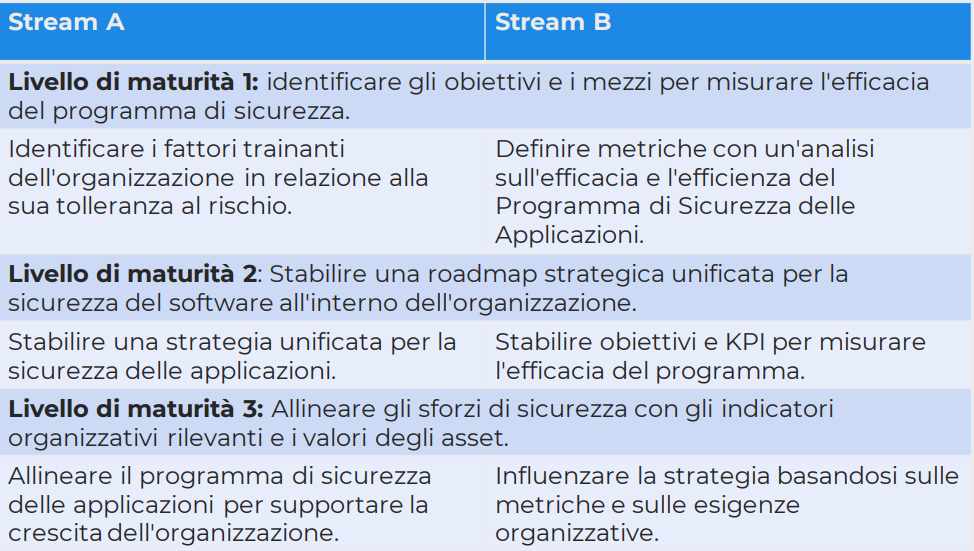
\includegraphics[width=6.26772in,height=4.33333in]{media/image13.png}

Attraverso le tecniche precedentemente dette andiamo a individuare
diversi punti nel dominio del tempo e dell'ampiezza.

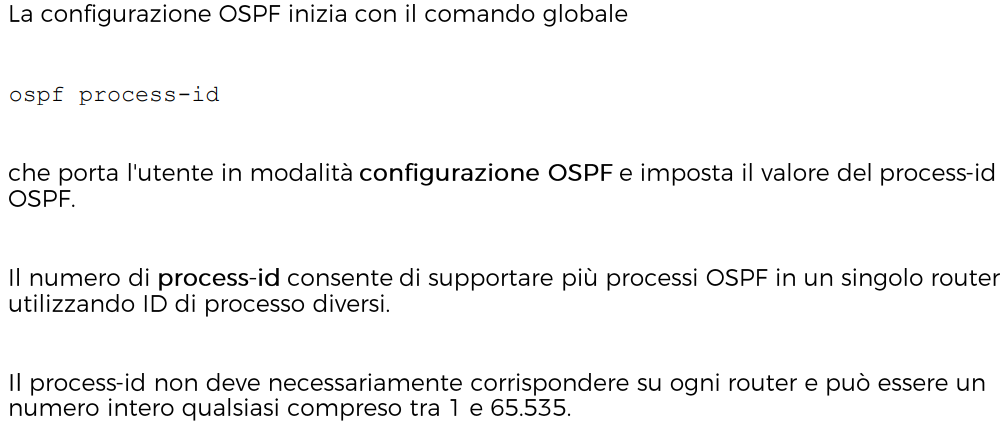
\includegraphics[width=5.55208in,height=2.30208in]{media/image4.png}

Alla fine codifichiamo con una sequenza di bit il suono.

Per avere un segnale audio più simile all'originale dobbiamo avere
intervalli di campionamento più piccoli (in modo da perdere meno segnale
in mezzo a essi) e avere abbastanza bit nella fase di quantizzazione per
descrivere il suono; ovviamente maggiore accuratezza significa maggior
quantità di memoria occupata\textbf{.}

\textbf{ALGEBRA BOOLEANA}

È un sistema di logica matematica a due stati, dove le variabili possono
assumere solo due stati: vero (1) o falso (0).

Si studia l'algebra booleana poiché le funzioni dell'algebra booleana
sono isomorfe ai circuiti digitali: un circuito digitale può essere
espresso tramite un'espressione booleana e viceversa.

Una funzione booleana ha una o più variabili in input e fornisce
risultati che dipendono solo da queste variabili. Quindi una funzione
booleana con \emph{n} variabili in input avrà solo \(2^{n}\)
combinazioni possibili.

Qualsiasi funzione può essere espressa con l'ausilio di \textbf{AND},
\textbf{OR} e \textbf{NOT} detto ciò è possibile tradurre qualsiasi
espressione in un circuito.

Qui i significati degli operatori:

\begin{longtable}[]{@{}
  >{\raggedright\arraybackslash}p{(\linewidth - 4\tabcolsep) * \real{0.3333}}
  >{\raggedright\arraybackslash}p{(\linewidth - 4\tabcolsep) * \real{0.3333}}
  >{\raggedright\arraybackslash}p{(\linewidth - 4\tabcolsep) * \real{0.3333}}@{}}
\toprule\noalign{}
\begin{minipage}[b]{\linewidth}\centering
\textbf{AND}
\end{minipage} & \begin{minipage}[b]{\linewidth}\centering
\emph{prodotto logico}
\end{minipage} & \begin{minipage}[b]{\linewidth}\centering
=1 solo se tutti 1
\end{minipage} \\
\begin{minipage}[b]{\linewidth}\centering
\textbf{OR}
\end{minipage} & \begin{minipage}[b]{\linewidth}\centering
\emph{somma logica}
\end{minipage} & \begin{minipage}[b]{\linewidth}\centering
=1 se almeno un 1
\end{minipage} \\
\begin{minipage}[b]{\linewidth}\centering
\textbf{NOT}
\end{minipage} & \begin{minipage}[b]{\linewidth}\centering
\emph{valore opposto}
\end{minipage} & \begin{minipage}[b]{\linewidth}\centering
se A=1 allora Ā=0
\end{minipage} \\
\midrule\noalign{}
\endhead
\bottomrule\noalign{}
\endlastfoot
\end{longtable}

\subparagraph{\texorpdfstring{\emph{Teoremi}}{Teoremi}}\label{teoremi}

Esistono proprietà per semplificare le espressioni booleane, ecco quali:

\begin{longtable}[]{@{}
  >{\raggedright\arraybackslash}p{(\linewidth - 4\tabcolsep) * \real{0.3333}}
  >{\raggedright\arraybackslash}p{(\linewidth - 4\tabcolsep) * \real{0.3333}}
  >{\raggedright\arraybackslash}p{(\linewidth - 4\tabcolsep) * \real{0.3333}}@{}}
\toprule\noalign{}
\begin{minipage}[b]{\linewidth}\centering
\textbf{Nome legge}
\end{minipage} & \begin{minipage}[b]{\linewidth}\centering
Forma \textbf{AND}
\end{minipage} & \begin{minipage}[b]{\linewidth}\centering
Forma \textbf{OR}
\end{minipage} \\
\begin{minipage}[b]{\linewidth}\centering
\emph{Identità}
\end{minipage} & \begin{minipage}[b]{\linewidth}\centering
1A = A
\end{minipage} & \begin{minipage}[b]{\linewidth}\centering
0 + A = A
\end{minipage} \\
\begin{minipage}[b]{\linewidth}\centering
\emph{Annullamento}
\end{minipage} & \begin{minipage}[b]{\linewidth}\centering
0A = 0
\end{minipage} & \begin{minipage}[b]{\linewidth}\centering
1 + A = 1
\end{minipage} \\
\begin{minipage}[b]{\linewidth}\centering
\emph{Impotenza}
\end{minipage} & \begin{minipage}[b]{\linewidth}\centering
AA = A
\end{minipage} & \begin{minipage}[b]{\linewidth}\centering
A + A = A
\end{minipage} \\
\begin{minipage}[b]{\linewidth}\centering
\emph{Inverso}
\end{minipage} & \begin{minipage}[b]{\linewidth}\centering
AĀ = 0
\end{minipage} & \begin{minipage}[b]{\linewidth}\centering
A + Ā = 1
\end{minipage} \\
\begin{minipage}[b]{\linewidth}\centering
\emph{Commutativa}
\end{minipage} & \begin{minipage}[b]{\linewidth}\centering
AB = BA
\end{minipage} & \begin{minipage}[b]{\linewidth}\centering
A + B = B + A
\end{minipage} \\
\begin{minipage}[b]{\linewidth}\centering
\emph{Associativa}
\end{minipage} & \begin{minipage}[b]{\linewidth}\centering
(AB)C = A(BC)
\end{minipage} & \begin{minipage}[b]{\linewidth}\centering
(A + B) + C = A + (B + C)
\end{minipage} \\
\begin{minipage}[b]{\linewidth}\centering
\emph{Distributiva}
\end{minipage} & \begin{minipage}[b]{\linewidth}\centering
A + BC = (A + B)(A + C)
\end{minipage} & \begin{minipage}[b]{\linewidth}\centering
A(B + C) = AB + AC
\end{minipage} \\
\begin{minipage}[b]{\linewidth}\centering
\emph{Assorbimento}
\end{minipage} & \begin{minipage}[b]{\linewidth}\centering
A(A + B) = A
\end{minipage} & \begin{minipage}[b]{\linewidth}\centering
A + AB = A
\end{minipage} \\
\begin{minipage}[b]{\linewidth}\centering
\emph{De Morgan}
\end{minipage} & \begin{minipage}[b]{\linewidth}\centering
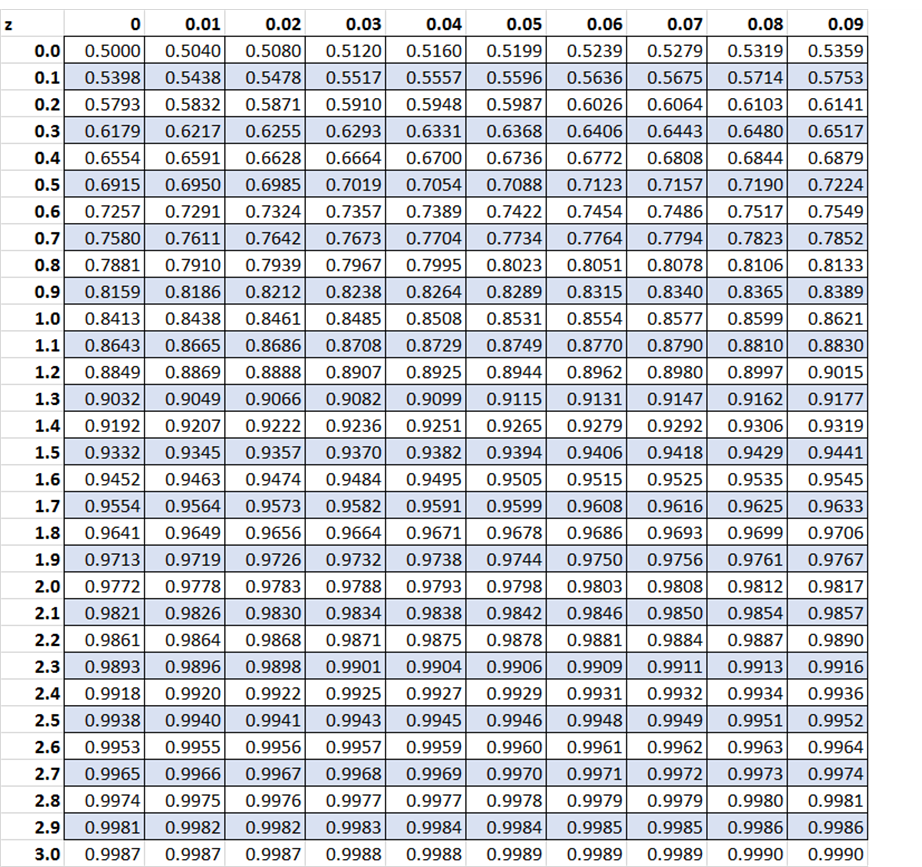
\includegraphics[width=0.85827in,height=0.22962in]{media/image9.png}
\end{minipage} & \begin{minipage}[b]{\linewidth}\centering
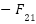
\includegraphics[width=0.88976in,height=0.24129in]{media/image14.png}
\end{minipage} \\
\begin{minipage}[b]{\linewidth}\centering
\emph{Assorbimento 2°}
\end{minipage} & \begin{minipage}[b]{\linewidth}\centering
A + ĀB = A + B
\end{minipage} & \begin{minipage}[b]{\linewidth}\centering
\textbackslash\textbackslash{}
\end{minipage} \\
\midrule\noalign{}
\endhead
\bottomrule\noalign{}
\endlastfoot
\end{longtable}

Per \emph{verificare} le leggi e teoremi bisogna creare tabelle di
verità, es di dimostrazione della 2° legge dell'assorbimento:

\begin{longtable}[]{@{}
  >{\raggedright\arraybackslash}p{(\linewidth - 8\tabcolsep) * \real{0.1296}}
  >{\raggedright\arraybackslash}p{(\linewidth - 8\tabcolsep) * \real{0.1279}}
  >{\raggedright\arraybackslash}p{(\linewidth - 8\tabcolsep) * \real{0.2608}}
  >{\raggedright\arraybackslash}p{(\linewidth - 8\tabcolsep) * \real{0.2791}}
  >{\raggedright\arraybackslash}p{(\linewidth - 8\tabcolsep) * \real{0.2026}}@{}}
\toprule\noalign{}
\begin{minipage}[b]{\linewidth}\centering
\textbf{A}
\end{minipage} & \begin{minipage}[b]{\linewidth}\centering
\textbf{B}
\end{minipage} & \begin{minipage}[b]{\linewidth}\centering
\textbf{Ā AND B}
\end{minipage} & \begin{minipage}[b]{\linewidth}\centering
\textbf{Ā AND B + A}
\end{minipage} & \begin{minipage}[b]{\linewidth}\centering
\textbf{A + B}
\end{minipage} \\
\begin{minipage}[b]{\linewidth}\centering
0
\end{minipage} & \begin{minipage}[b]{\linewidth}\centering
0
\end{minipage} & \begin{minipage}[b]{\linewidth}\centering
0
\end{minipage} & \begin{minipage}[b]{\linewidth}\centering
0
\end{minipage} & \begin{minipage}[b]{\linewidth}\centering
0
\end{minipage} \\
\begin{minipage}[b]{\linewidth}\centering
0
\end{minipage} & \begin{minipage}[b]{\linewidth}\centering
1
\end{minipage} & \begin{minipage}[b]{\linewidth}\centering
1
\end{minipage} & \begin{minipage}[b]{\linewidth}\centering
1
\end{minipage} & \begin{minipage}[b]{\linewidth}\centering
1
\end{minipage} \\
\begin{minipage}[b]{\linewidth}\centering
1
\end{minipage} & \begin{minipage}[b]{\linewidth}\centering
0
\end{minipage} & \begin{minipage}[b]{\linewidth}\centering
0
\end{minipage} & \begin{minipage}[b]{\linewidth}\centering
1
\end{minipage} & \begin{minipage}[b]{\linewidth}\centering
1
\end{minipage} \\
\begin{minipage}[b]{\linewidth}\centering
1
\end{minipage} & \begin{minipage}[b]{\linewidth}\centering
1
\end{minipage} & \begin{minipage}[b]{\linewidth}\centering
0
\end{minipage} & \begin{minipage}[b]{\linewidth}\centering
1
\end{minipage} & \begin{minipage}[b]{\linewidth}\centering
1
\end{minipage} \\
\midrule\noalign{}
\endhead
\bottomrule\noalign{}
\endlastfoot
\end{longtable}

↑ ↑

Essendo queste due parti uguali il teorema è verificato

\subparagraph{\texorpdfstring{\emph{Tabelle di
verità}}{Tabelle di verità}}\label{tabelle-di-verituxe0}

Con l'utilizzo delle tabelle di verità posso arrivare a una espressione
andando a individuare quali combinazioni con output 1 rappresentano quel
risultato.

Questo tipo di espressioni si chiamano in \emph{prima forma canonica,}
per arrivare a questa forma è necessario:

\begin{enumerate}
\def\labelenumi{\arabic{enumi}.}
\item
  Identificare le righe in output (\textbf{V}) con risultato 1;
\item
  in queste righe scrivere la configurazione delle variabili che le
  definiscono (saranno in \textbf{AND} tra loro);
\item
  collegare tutte le configurazioni con l'\textbf{OR}.
\end{enumerate}

Es:

\begin{longtable}[]{@{}
  >{\raggedright\arraybackslash}p{(\linewidth - 6\tabcolsep) * \real{0.2719}}
  >{\raggedright\arraybackslash}p{(\linewidth - 6\tabcolsep) * \real{0.2719}}
  >{\raggedright\arraybackslash}p{(\linewidth - 6\tabcolsep) * \real{0.2396}}
  >{\raggedright\arraybackslash}p{(\linewidth - 6\tabcolsep) * \real{0.2166}}@{}}
\toprule\noalign{}
\begin{minipage}[b]{\linewidth}\centering
\textbf{X}
\end{minipage} & \begin{minipage}[b]{\linewidth}\centering
\textbf{Y}
\end{minipage} & \begin{minipage}[b]{\linewidth}\centering
\textbf{Z}
\end{minipage} & \begin{minipage}[b]{\linewidth}\centering
\textbf{\hl{V}}
\end{minipage} \\
\begin{minipage}[b]{\linewidth}\centering
0
\end{minipage} & \begin{minipage}[b]{\linewidth}\centering
0
\end{minipage} & \begin{minipage}[b]{\linewidth}\centering
0
\end{minipage} & \begin{minipage}[b]{\linewidth}\centering
\hl{0}
\end{minipage} \\
\begin{minipage}[b]{\linewidth}\centering
\hl{0}
\end{minipage} & \begin{minipage}[b]{\linewidth}\centering
\hl{0}
\end{minipage} & \begin{minipage}[b]{\linewidth}\centering
\hl{1}
\end{minipage} & \begin{minipage}[b]{\linewidth}\centering
\hl{1}
\end{minipage} \\
\begin{minipage}[b]{\linewidth}\centering
\hl{0}
\end{minipage} & \begin{minipage}[b]{\linewidth}\centering
\hl{1}
\end{minipage} & \begin{minipage}[b]{\linewidth}\centering
\hl{0}
\end{minipage} & \begin{minipage}[b]{\linewidth}\centering
\hl{1}
\end{minipage} \\
\begin{minipage}[b]{\linewidth}\centering
0
\end{minipage} & \begin{minipage}[b]{\linewidth}\centering
1
\end{minipage} & \begin{minipage}[b]{\linewidth}\centering
1
\end{minipage} & \begin{minipage}[b]{\linewidth}\centering
\hl{0}
\end{minipage} \\
\begin{minipage}[b]{\linewidth}\centering
\hl{1}
\end{minipage} & \begin{minipage}[b]{\linewidth}\centering
\hl{0}
\end{minipage} & \begin{minipage}[b]{\linewidth}\centering
\hl{0}
\end{minipage} & \begin{minipage}[b]{\linewidth}\centering
\hl{1}
\end{minipage} \\
\begin{minipage}[b]{\linewidth}\centering
1
\end{minipage} & \begin{minipage}[b]{\linewidth}\centering
0
\end{minipage} & \begin{minipage}[b]{\linewidth}\centering
1
\end{minipage} & \begin{minipage}[b]{\linewidth}\centering
\hl{0}
\end{minipage} \\
\begin{minipage}[b]{\linewidth}\centering
1
\end{minipage} & \begin{minipage}[b]{\linewidth}\centering
1
\end{minipage} & \begin{minipage}[b]{\linewidth}\centering
0
\end{minipage} & \begin{minipage}[b]{\linewidth}\centering
\hl{0}
\end{minipage} \\
\begin{minipage}[b]{\linewidth}\centering
\hl{1}
\end{minipage} & \begin{minipage}[b]{\linewidth}\centering
\hl{1}
\end{minipage} & \begin{minipage}[b]{\linewidth}\centering
\hl{1}
\end{minipage} & \begin{minipage}[b]{\linewidth}\centering
\hl{1}
\end{minipage} \\
\midrule\noalign{}
\endhead
\bottomrule\noalign{}
\endlastfoot
\end{longtable}

Le righe evidenziate sono quelle con risultato (\textbf{V}) 1, quindi
quelle che ci interessano. Ora andiamo a scrivere le loro
configurazioni:

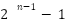
\includegraphics[width=0.3937in,height=0.2874in]{media/image10.png}

Riga 1 →

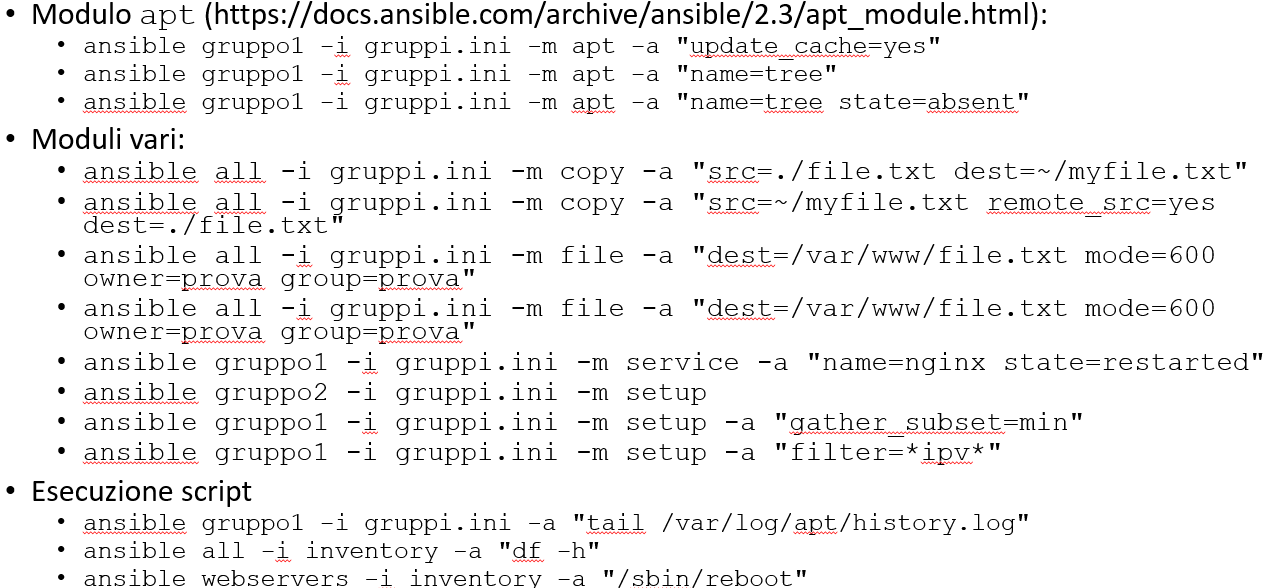
\includegraphics[width=0.3937in,height=0.25054in]{media/image2.png}

Riga 2 →
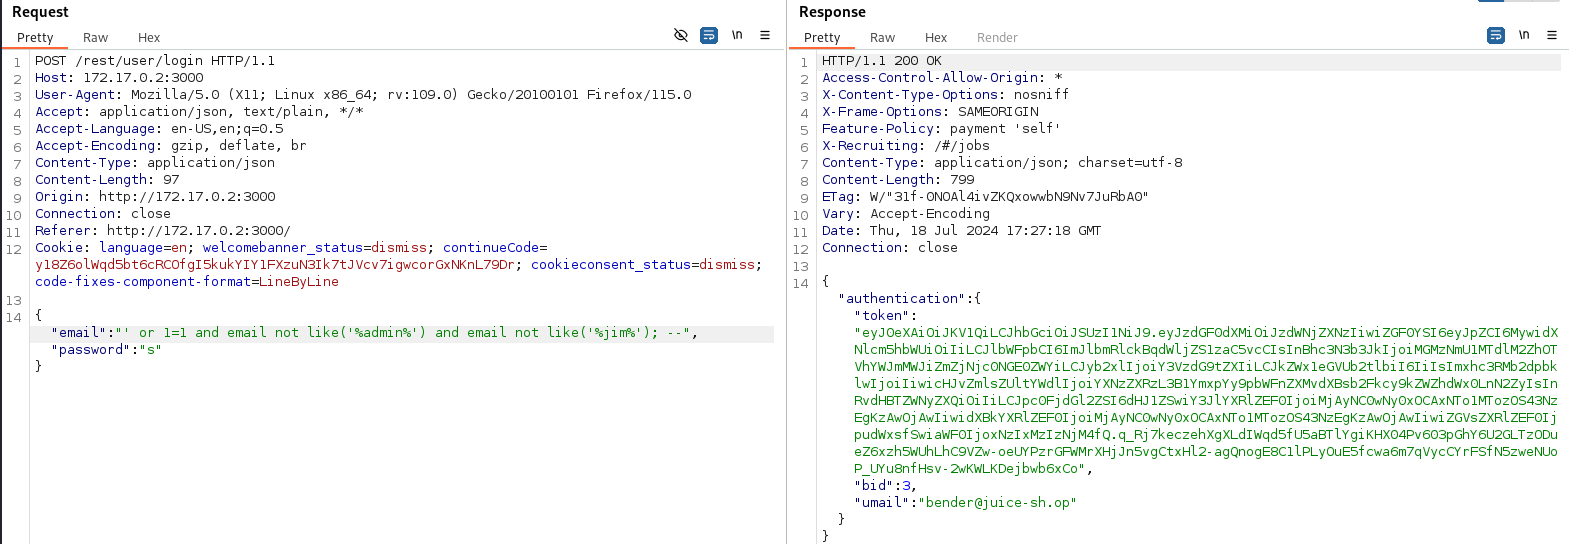
\includegraphics[width=2.41339in,height=0.31496in]{media/image16.png}

\textbf{Risultato finale} →
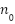
\includegraphics[width=0.3937in,height=0.25197in]{media/image17.png}

Riga 4 →

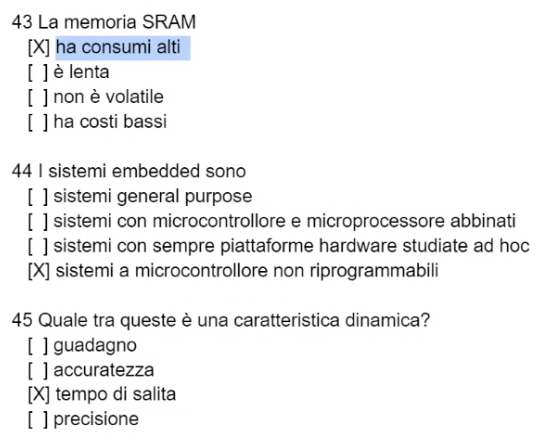
\includegraphics[width=0.3937in,height=0.25197in]{media/image8.png}

Riga 7 →

Due funzioni con ugual output si dicono equivalenti, andare a
determinare la più semplice funzione booleana equivalente alla funzione
data facilita l'interpretazione della funzione stessa e permette di
semplificare anche i circuiti logici corrispondenti.

\textbf{ARCHITETTURA DEI CALCOLATORI}

Un calcolatore è un sistema composto da un numero elevato di componenti,
il modello base è rappresentato dalla macchina di Von Neumann, composto
da:

\begin{itemize}
\item
  \emph{CPU;}
\item
  \emph{Memoria;}
\item
  \emph{Periferiche;}
\item
  \emph{Bus.}
\end{itemize}

\paragraph{BUS}\label{bus}

Gestito dalla CPU (master) e nessun'altra unità (slave) può accedervi
autonomamente. Permette la comunicazione tra periferiche, CPU, cache,
memoria, ecc.

I Bus possono essere:

\begin{itemize}
\item
  \emph{bus dati}: costituiti da \(2^{n}\) linee fisiche, passano i dati
  I/O della CPU;
\item
  \emph{bus degli indirizzi}: determina l'indirizzo di memoria dove si
  andrà a leggere o scrivere;
\item
  \emph{bus di controllo}: indica cosa fare nell'indirizzo di memoria (
  andare a leggere o scrivere).
\end{itemize}

\paragraph{SCHEDA MADRE}\label{scheda-madre}

Contiene l\textquotesingle alloggiamento CPU, i bus, i connettori di
memoria, i connettori I/O, ecc.

La scheda madre controlla un insieme di chip detti \emph{chipset}.

Dentro la Motherboard sono presenti dei connettori PCI (Peripheral
Component Interconnect) dove è possibile posizionare schede specifiche
come la GPU o l\textquotesingle Ethernet card.

\paragraph{CPU}\label{cpu}

Il cuore operativo del calcolatore, può essere chiamato anche processore
o microprocessore, con il compito di eseguire i programmi presenti in
RAM andando a leggere le loro istruzioni in sequenza.

È composta da:

\begin{itemize}
\item
  \emph{Unità di controllo}: legge le istruzioni in RAM;
\item
  \emph{ALU}: esegue le operazioni (AND, OR, \ldots) necessarie per
  l'esecuzione;
\item
  \emph{Registri}: sono celle di memoria molto piccole dove si salvano
  temporaneamente i risultati delle operazioni, in oltre sono proprio i
  registri che determinano il tipo della CPU (32 o 64 bit).
\end{itemize}

\begin{quote}
Al momento non si va oltre i 64 bit per via dei problemi di
retrocompatibilità che ci potrebbero essere con i programmi scritti in
128 bit.

I registri di dividono in:
\end{quote}

\begin{itemize}
\item
  \textbf{PC} (Program Counter): Conserva l'indirizzo di memoria della
  prossima istruzione da seguire;
\item
  \textbf{IR} (Instruction Register) contiene copia della codifica
  dell'istruzione da eseguire;
\item
  \textbf{MAR} (Memory Address Register): contiene l'indirizzo di
  memoria dove bisogna leggere/scrivere.
\item
  \textbf{MDR} (Memory Data Register): contiene
  l\textquotesingle informazione appena letta in memoria;
\item
  \textbf{PSW} (Processor Status Word): indica in che stato è il
  programma.
\end{itemize}

La CPU lavora in modo ciclico andando a ripetere le operazioni qui sotto
elencate fino alla fine dell'esecuzione:

\begin{itemize}
\item
  \emph{Caricamento} (\textbf{Fetch}): acquisizione dalla memoria di
  un'istruzione del programma;
\item
  \emph{Decodifica} (\textbf{Decode}): identificazione del tipo di
  operazione da eseguire;
\item
  \emph{Esecuzione} (\textbf{Execute}): effettuazione delle operazioni
  corrispondenti all'istruzione.
\end{itemize}

Il ciclo di esecuzione con le seguenti operazioni è:

\begin{enumerate}
\def\labelenumi{\arabic{enumi}.}
\item
  Segnale di avvio: il \textbf{PC} viene inizializzato con l'indirizzo
  della prima istruzione da eseguire {[} fatto una volta sola {]};
\item
  la CPU imposta \textbf{MAR} ← \textbf{PC};
\item
  viene selezionata la cella da leggere, il contenuto viene inviato sul
  bus;
\item
  la CPU imposta \textbf{IR} ← \textbf{MAR};
\item
  la CPU incrementa il \textbf{PC} in modo che punti alla prossima
  istruzione;
\item
  la CPU esamina il \textbf{IR} e determina le operazioni da svolgere;
\item
  tutte le unità interessate all'esecuzione vengono comandate;
\item
  al fine del ciclo la CPU torna al punto \emph{\textbf{2}}.
\end{enumerate}

I colori dei numeri rappresentano le fasi di Fetch, Decode e Execute.

\subparagraph{\texorpdfstring{\emph{Linguaggio macchina e
assembly}}{Linguaggio macchina e assembly}}\label{linguaggio-macchina-e-assembly}

\textbf{Il linguaggio macchina} è un linguaggio comprensibile
direttamente dal processore della macchina.

\textbf{L'assembler} invece è la versione simbolica del linguaggio
macchina in cui i nomi delle operazioni e degli operandi sono indicati
con codici simbolici; è usato per parlare direttamente con la macchina.

Esempio programma assembler e traduzione in binario:

X = Y + 2 → LOAD Y, R1 carica Y in R (dove R è un indirizzo interno al
processore {[}cache{]})

ADD 2, R1 aggiunge 2 al contenuto di R1

STORE R1, X scrive il contenuto di R1 in X (dove X, così come Y, è un
indirizzo di memoria)

Ogni operazione viene codificata (che è sempre un Word o multipli)
diversamente in base al formato stabilito dal costruttore dell'hardware,
esempio:

\begin{longtable}[]{@{}
  >{\raggedright\arraybackslash}p{(\linewidth - 8\tabcolsep) * \real{0.2492}}
  >{\raggedright\arraybackslash}p{(\linewidth - 8\tabcolsep) * \real{0.2160}}
  >{\raggedright\arraybackslash}p{(\linewidth - 8\tabcolsep) * \real{0.1628}}
  >{\raggedright\arraybackslash}p{(\linewidth - 8\tabcolsep) * \real{0.1695}}
  >{\raggedright\arraybackslash}p{(\linewidth - 8\tabcolsep) * \real{0.2026}}@{}}
\toprule\noalign{}
\begin{minipage}[b]{\linewidth}\centering
\textbf{Codice operativo}
\end{minipage} & \begin{minipage}[b]{\linewidth}\centering
\textbf{Modo 1}
\end{minipage} & \begin{minipage}[b]{\linewidth}\centering
\textbf{Op1}
\end{minipage} & \begin{minipage}[b]{\linewidth}\centering
\textbf{Modo 2}
\end{minipage} & \begin{minipage}[b]{\linewidth}\centering
\textbf{Op2}
\end{minipage} \\
\midrule\noalign{}
\endhead
\bottomrule\noalign{}
\endlastfoot
\end{longtable}

Dove:

\begin{enumerate}
\def\labelenumi{\arabic{enumi}.}
\item
  Il \textbf{codice operativo} {[} 4 bit {]}: indica la codifica
  dell'operazione da fare (es: ADD 0001, LOAD 0110, ecc);
\item
  Il \textbf{Modo 1/Modo 2} {[} 2 bit {]}: indica a cosa si riferisce
  \emph{Op1/Op2} (es: se è 00 allora Op1/Op2 è un numero di registro o
  01 allora Op1/Op2 è un indirizzo, ecc);
\item
  I'\textbf{Op1/Op2} {[} 12 bit {]}: è quel qualcosa indicato dal suo
  modo.
\end{enumerate}

Quindi ora la traduzione del programma precedente in linguaggio macchina
sarà:

\textbf{Modi}:

\begin{itemize}
\item
  \emph{00} = registro;
\item
  \emph{01} = memoria;
\item
  \emph{10} = immediato (è un dato).
\end{itemize}

\textbf{Cod. operativi}:

\begin{itemize}
\item
  \emph{ADD} = 0001;
\item
  \emph{LOAD} = 0110;
\item
  \emph{STORE} = 0111.
\end{itemize}

Traduzione:

\begin{longtable}[]{@{}
  >{\raggedright\arraybackslash}p{(\linewidth - 8\tabcolsep) * \real{0.2000}}
  >{\raggedright\arraybackslash}p{(\linewidth - 8\tabcolsep) * \real{0.2000}}
  >{\raggedright\arraybackslash}p{(\linewidth - 8\tabcolsep) * \real{0.2000}}
  >{\raggedright\arraybackslash}p{(\linewidth - 8\tabcolsep) * \real{0.2000}}
  >{\raggedright\arraybackslash}p{(\linewidth - 8\tabcolsep) * \real{0.2000}}@{}}
\toprule\noalign{}
\begin{minipage}[b]{\linewidth}\centering
0110
\end{minipage} & \begin{minipage}[b]{\linewidth}\centering
01
\end{minipage} & \begin{minipage}[b]{\linewidth}\centering
01101
\end{minipage} & \begin{minipage}[b]{\linewidth}\centering
00
\end{minipage} & \begin{minipage}[b]{\linewidth}\centering
00001 \textbf{{[}*{]}}
\end{minipage} \\
\begin{minipage}[b]{\linewidth}\centering
0001
\end{minipage} & \begin{minipage}[b]{\linewidth}\centering
10
\end{minipage} & \begin{minipage}[b]{\linewidth}\centering
00010
\end{minipage} & \begin{minipage}[b]{\linewidth}\centering
00
\end{minipage} & \begin{minipage}[b]{\linewidth}\centering
00001
\end{minipage} \\
\begin{minipage}[b]{\linewidth}\centering
0111
\end{minipage} & \begin{minipage}[b]{\linewidth}\centering
00
\end{minipage} & \begin{minipage}[b]{\linewidth}\centering
00001
\end{minipage} & \begin{minipage}[b]{\linewidth}\centering
01
\end{minipage} & \begin{minipage}[b]{\linewidth}\centering
11100
\end{minipage} \\
\midrule\noalign{}
\endhead
\bottomrule\noalign{}
\endlastfoot
\end{longtable}

\textbf{Ogni riga della tabella equivale ad una riga istruzione del
programma precedente.}

\textbf{{[}*{]}} essendo questo R1 per tradurlo in binario prendiamo
solo il numero (1 in questo caso).

\subparagraph{\texorpdfstring{\emph{ALU}}{ALU}}\label{alu}

Serve per effettuare operazioni di tipo aritmetico e logico booleano, un
bit di

ALU è così rappresentato:

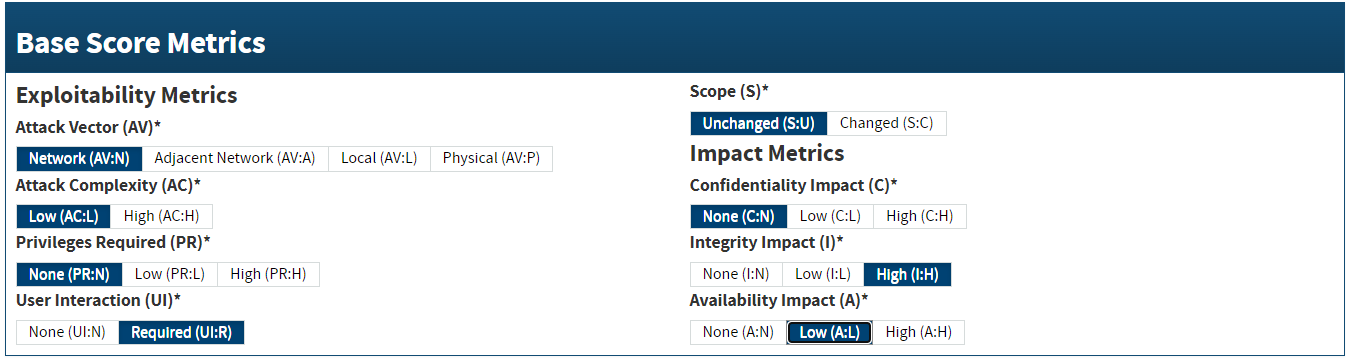
\includegraphics[width=4.46063in,height=2.35325in]{media/image26.jpg}

per rappresentare operazioni con più bit ne metto uno dietro l'altra.

Es:

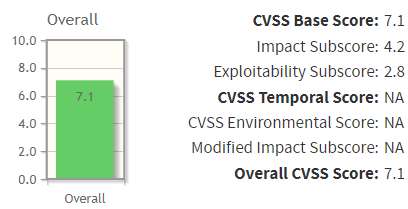
\includegraphics[width=3.56847in,height=6.77083in]{media/image27.jpg}

Qui possiamo vedere una somma 01+01, ogni ALU fa l'operazione della
posizione corrispondente, in questo caso la 1° ALU farà l'operazione fra
i numeri della posizione 0 (1+1) invece la 2° quelli della posizione 1
(0+0).

\paragraph{PROCESSORE}\label{processore}

\subparagraph{\texorpdfstring{\emph{Clock e
GHz}}{Clock e GHz}}\label{clock-e-ghz}

L'esecuzione di ogni processo viene misurata in \emph{clock}, cioè la
velocità del processore di eseguire operazioni.

L'esecuzione è sincrona, quindi prima di fare
l\textquotesingle operazione successiva è necessario finire la
precedente. Alla fine di ogni operazione c'è un \emph{tick}, misurato in
Hz (tick al secondo), che scandisce le varie istruzioni.

\subparagraph{\texorpdfstring{\emph{CISC vs
RISC}}{CISC vs RISC}}\label{cisc-vs-risc}

Nel mondo informatico esistono 2 correnti di pensiero sull'utilizzo
della CPU:

\begin{itemize}
\item
  \textbf{CISC}: in questo caso si decide di dare al processore più
  operazioni possibili alla CPU anche a scapito di avere
  \emph{\textbf{più cicli};}
\item
  \textbf{RISC}\emph{:} in questo caso si decide che per ogni ciclo
  viene eseguita una e una sola istruzione, quindi ci saranno
  \emph{\textbf{più istruzioni}}.
\end{itemize}

Nel \emph{RISC} tutte le istruzioni e le istruzioni macchina vengono
eseguite direttamente dall'hardware e viene utilizzato il pipelining e
parallelismo.

\subparagraph{\texorpdfstring{\emph{Pipelining}}{Pipelining}}\label{pipelining}

L'esecuzione di ogni istruzione viene suddivisa in più fasi
(\emph{stadi}) dove ognuna delle quali viene gestita da un hardware
dedicato.

Per far in modo che questo accada bisogna garantire che le istruzioni
non siano in conflitto (non devono dipendere l'una dall'altra).

\subparagraph{\texorpdfstring{\emph{Parallelismo}}{Parallelismo}}\label{parallelismo}

Ne esistono di 2 tipi:

\begin{enumerate}
\def\labelenumi{\arabic{enumi}.}
\item
  \textbf{a livello di istruzione}: più istruzioni vengono eseguite
  contemporaneamente all'interno della stessa CPU tramite tecniche di
  pipelining e processori superscalari;
\item
  \textbf{a livello di processore}: più CPU cooperano per la soluzione
  dello stesso problema, andando però ad abbandonare il modello Neumann.
\end{enumerate}

\subparagraph{\texorpdfstring{\emph{Prestazioni}}{Prestazioni}}\label{prestazioni}

Per calcolare il tempo di esecuzione abbiamo bisogno della seguente
formula:

\(T_{esecuzione} = T_{clock}*(\sum_{i = l}^{n}N_{i}*CPI_{I})\)

dove:

\begin{itemize}
\item
  Tclock : periodo di clock della macchina;
\item
  \(CPI_{I}\) : numero di clock per ogni istruzione di tipo i;
\item
  \(N_{i}\): numero di istruzioni di tipo i;
\end{itemize}

\paragraph{MEMORIE}\label{memorie}

È la capacità di memorizzare le informazioni del calcolatore, deve
essere veloce, capiente e persistente; per conciliare le diverse
caratteristiche esistono due categorie:

\begin{itemize}
\item
  \emph{memoria centrale} ( veloce ma non persistente, contiene i
  programmi in esecuzione);
\item
  \emph{memoria di massa} ( più lenta ma capiente e persistente).
\end{itemize}

\subparagraph{}\label{section-4}

\subparagraph{\texorpdfstring{\emph{Tecnologie e
struttura}}{Tecnologie e struttura}}\label{tecnologie-e-struttura}

Esistono diverse tecnologie usate ora e in passato per creare le
memorie:

\begin{itemize}
\item
  \emph{elettroniche} {[} mem. centrale {]}: veloci ma sempre
  alimentate, costo per bit elevato;
\item
  \emph{magnetiche} {[} mem. massa {]}: basso costo per bit ma non
  volatili, sono lente;
\item
  \emph{ottiche}: riscrivibili e utili alla grossa distribuzione.
\end{itemize}

La memoria centrale è strutturata in \emph{celle}, successione ordinata
di elementi binari raggruppati in unità minime, e ogni cella ha un
proprio \emph{indirizzo} ( si parte dallo 0).

\emph{Con K bit posso avere} \(2^{K}\) \emph{celle.}

\subparagraph{\texorpdfstring{\emph{Tipo di
accesso}}{Tipo di accesso}}\label{tipo-di-accesso}

Esistono quattro modi per accedere ad una cella di memoria, ogni modo
dipende dal tipo di memoria:

\begin{enumerate}
\def\labelenumi{\arabic{enumi}.}
\item
  accesso sequenziale {[} nastri {]}: prima di poter arrivare alla cella
  interessata devo leggere le celle precedenti;
\item
  accesso casuale {[} casuale {]}: il tempo di accesso è indipendente
  dalla posizione e costante per tutte le celle;
\item
  accesso misto {[} dischi {]}: si accede in prossimità del dato e si
  procede in modo sequenziale;
\item
  accesso associativo {[} cache {]}: le celle si selezionano in base al
  tipo di dato contenuto, si usa per permettere alla CPU di avere subito
  i dati di un determinato processo.
\end{enumerate}

Si può accedere alla memoria centrale mediante il registro MAR e si
prelevano/scrivono dati tramite l'MDR in base al segnale di
lettura/scrittura definito dal bus di controllo.

\subparagraph{\texorpdfstring{\emph{RAM vs ROM vs
Flash}}{RAM vs ROM vs Flash}}\label{ram-vs-rom-vs-flash}

\textbf{Memoria RAM} (Random Access Memory): ad accesso casuale
realizzata mediante circuiti a semiconduttori, di tipo volatile;

\textbf{Memoria ROM} (Read-Only Memory): non volatile, scritta al
momento della produzione e che non può essere cancellata. Contiene il
BIOS;

\textbf{Memorie FLASH}: elettroniche non volatili ma riscrivibili.

\subparagraph{\texorpdfstring{\emph{Tipi di RAM}
}{Tipi di RAM }}\label{tipi-di-ram}

I chip di memoria non vengono venduti singolarmente ma sono normalmente
organizzati su schede stampate. I principali formati sono:

\begin{itemize}
\item
  \textbf{SIMM} (Single Inline Memory Module) : utilizza moduli DRAM
  quindi immagazzina ogni bit in un diverso condensatore (acceso 0
  altrimenti 1), se il condensatore perde la carica,
  l\textquotesingle informazione è perduta;
\item
  \textbf{DIMM} (Dual Inline Memory Module): utilizzano SDRAM e i
  connettori si trovano su entrambe i lati della scheda;
\item
  \textbf{SO-DIMM} (Small Outline Dual In-line Memory Module): sono
  semplicemente più piccoli e costano di meno.
\end{itemize}

Attualmente sul mercato esistono \emph{due tipi distinti} di RAM: quelle
di tipo \textbf{SDR} (Single Data Rate) e quelle \textbf{DDR} (Double
Data Rate). Quest'ultime (DDR) possono trasferire un byte sia sul fronte
di salita che su quello di discesa del clock (lavorano il doppio
rispetto alle SDR che fanno un'operazione a colpo di clock).

Le DDR sono arrivate alle Gen 5 e non sono retrocompatibili.

\subparagraph{\texorpdfstring{\emph{Tipi di
ROM}}{Tipi di ROM}}\label{tipi-di-rom}

Le ROM esistenti sono:

\begin{itemize}
\item
  \textbf{ROM} (Read Only Memory): uniche veramente di sola lettura;
\item
  \textbf{PROM} (Programmable Read Only Memory): programmabili una sola
  volta;
\item
  \textbf{EPROM} (Erasable Programmable Read Only Memory): riprogrammate
  con apparecchiature speciali;
\item
  \textbf{EEPROM} (Electrically Erasable Programmable Read Only Memory).
\end{itemize}

\subparagraph{\texorpdfstring{\emph{Cache}}{Cache}}\label{cache}

Per ovviare al problema di aspettare che l'informazione arrivi dalla
memoria alla CPU si è creata una memoria super veloce vicina al
processore, denominata \emph{cache}.

In questa memoria si caricano tutte quelle informazioni che la CPU avrà
bisogno per un determinato processo andando a vedere qual è l'ultima
cella utilizzata.

Al momento ne esistono 3 livelli:

\begin{enumerate}
\def\labelenumi{\arabic{enumi}.}
\item
  \textbf{L1 -- Cache di livello 1}, fa fisicamente parte del chip del
  microprocessore. Molto piccola e molto veloce;
\item
  \textbf{L2 -- Cache di livello 2}, prima sulla scheda madre, adesso è
  nel core;
\item
  \textbf{L3 -- Cache di livello 3}, è completamente condivisa tra i
  core dell'elaboratore.
\end{enumerate}

\subparagraph{\texorpdfstring{\emph{Memorie di
massa}}{Memorie di massa}}\label{memorie-di-massa}

Nastri

Le prime memorie di massa create furono i nastri magnetici, permettono
solo accesso sequenziale ai dati e i dati vengono scritti
trasversalmente rispetto alla direzione.

Floppy Disk

Il Floppy disk è stato il primo supporto magnetico con accesso diretto
ai dati. I floppy disk possono memorizzare fino a 1,44 MB, il
funzionamento è simile a quello dell'hard disk.

Dischi magnetici (HDD)

Dispositivo elettromeccanico per la conservazione di informazioni sotto
forma magnetica, su \emph{supporto rotante} a forma di piatto su cui
agiscono delle testine di lettura/scrittura.

La \emph{testina} contenente un induttore ed è sospesa sopra la
superficie e viene sostenuta da un cuscino d'aria.

È possibile \emph{partizionare} il disco per dividere un unico HDD in
più parti logiche.

\textbf{Un hard disk è strutturato} per registrare dati su cilindri,
\emph{tracce} (sequenza circolare di bit) e \emph{settori} (composto da
preambolo, dati e codice errore).

\textbf{Per scrivere e leggere si usano due testine diverse}, in
\emph{scrittura} quando la corrente negativa o positiva passa attraverso
la testina, viene magnetizzata la superficie sotto la testina, invece in
\emph{lettura} quando una testina passa sopra un'area magnetizzata viene
indotta una corrente positiva o negativa nella testina: questo permette
di rileggere i bit memorizzati precedentemente.

\textbf{La capacità di memorizzazione} dipende principalmente dalla
densità di registrazione, quindi quante informazioni possono essere
immagazzinate in una determinata area.

\textbf{Le prestazioni} degli hard disk dipendono da:

\begin{itemize}
\item
  \emph{Seek time}: è il tempo necessario per spostare le testine sul
  cilindro desiderato;
\item
  \emph{Latency time}: il tempo necessario affinché il settore
  interessato passi sotto la testina (definito dalla velocità di
  rotazione del disco).
\end{itemize}

Dischi a stato solido (SDD)

Non hanno veramente dei dischi fisici ma sono basati su
\textbf{componenti elettronici} composti da chip \emph{NAND}, cioè
insieme di celle che includono un transistor MOSFET capace di
memorizzare in una sola cella più combinazioni di 0 e 1 (e non solo
true/false, 0/1) questo è possibile guardando la tensione elettrica data
ad una cella, per questo sono molto veloci ma la loro capacità di tenere
informazioni scende con il tempo.

Le memorie sono \textbf{classificate} da quanti valori di bit possono
essere conservati, alcuni esempi sono:

\begin{itemize}
\item
  SLC (single level cell, un bit): un solo bit per cella (0/1);
\item
  MLC (multi-level cell, due bit): 2 bit per cella (00/01/10/11);
\item
  TLC (triple-level cell, tre bit): 3 bit per cella
  (000/001/010/011/100/\ldots);
\item
  QLC (quad-level cell, quattro bit) 4 bit per cella
  (0000/0001/0010/0011/0100/\ldots).
\end{itemize}

Più si aumentano le combinazioni più il range di Volt necessari per
rappresentare i valori si abbassa e quindi è più possibile, con il
passare del tempo, che i valori diventino meno precisi.

Dischi ottici (CD)

Informazioni \textbf{codificate} per mezzo di \emph{fori} (Pit)
alternati con \emph{zone piane} (Land) lungo un'unica spirale. Un
passaggio PitLand o Land-Pit codifica un 1 invece l'assenza di
variazioni codifica lo 0.

La \textbf{lettura} avviene a tramite un raggio laser che viene riflesso
diversamente al passaggio su pit e land.

Lungo la spirale \textbf{i dati sono memorizzati con la stessa densità},
quindi il CD ruota con velocità angolare variabile per mantenere la
medesima velocità lineare nelle diverse aree del CD.

I dischi possono suddividersi in:

\begin{itemize}
\item
  \textbf{CD-ROM} (Compact Disc-Read Only Memory): utilizzano la
  tecnologia dei CD per memorizzare dati informatici, ogni byte viene
  \emph{codificato da un simbolo di 14 bit}, raggruppati poi in
  \emph{Frame}(gruppo di 42 simboli) e a loro volta in Settori (gruppo
  di 98 frame);
\item
  \textbf{CD-R} (Compact Disc-Recordable): sono registrabili dagli
  utenti senza l'utilizzo dello stampo, la riflettività di pit e land
  viene ottenuta ``bruciando'', tramite un raggio laser, uno strato di
  materiale colorato inserito tra il policarbonato e lo strato
  riflettente;
\item
  \textbf{CD-RW}: dischi riscrivibili molto simili come concetto a
  quelli registrabili ma possiedono la possibilità di essere cancellati;
\item
  \textbf{DVD} (Digital Video Disk o Digital Versatile Disk): Pit più
  piccoli, spirale più serrata e raggio laser rosso. Più capienti,
  veloci e con la possibilità di scrivere su due strati (tecnologia con
  doppio strato).
\end{itemize}

\begin{quote}
Altri standard DVD: DVD-R, DVD+R e DVD-RAM.
\end{quote}

\textbf{SISTEMI OPERATIVI}

\paragraph{DEFINIZIONI}\label{definizioni}

Un \textbf{sistema operativo} è un \emph{insieme di programmi}
(software) che \emph{gestiscono l'hardware}, fornendo una
\emph{piattaforma ai programmi} applicativi e agisce da intermediario
tra l'utente e la struttura fisica del calcolatore.

Il S.O. si colloca fra l'hardware e il software o comunque ciò che vede
e tocca l'utente, ha il compito di assegnare le risorse e decidere chi
userà la CPU e per quanto tempo.

Un'altro compito del S.O. è quello di generalizzare le caratteristiche
fisiche fino a renderle virtuali, andando anche a superare i limiti
fisici di certe parti del calcolatore.

Un altro modo di definire il sistema operativo è quello di considerarlo
come quello strato di software che fornisce a programmi e applicazioni
una macchina virtuale attraverso la quale accedere alle risorse hardware
del computer. Infatti fornisce agli sviluppatori di software la
possibilità di usare API semplici che nascondono le caratteristiche
dell'hardware.

\paragraph{STORIA}\label{storia}

Dal primo S.O. ad adesso sono passati molti anni, ecco come vengono
divisi:

\begin{enumerate}
\def\labelenumi{\arabic{enumi}.}
\item
  \emph{1° Gen {[}45-55{]}}: in questo periodo venivano usate macchine a
  valvole gestite con codici scritti su schede perforate, ancora non
  esiste il concetto di Sistema Operativo ed ogni programma era
  auto-contenuto;
\item
  \emph{2° Gen {[}55-65{]}}: i transistor vengono implementati nei
  computer e vengono identificati due nuovi ruoli:
\end{enumerate}

\begin{itemize}
\item
  Programmatore (con schede perforate e assembly);
\item
  Operatore (che esegue il job o programma).
\end{itemize}

\begin{quote}
Al momento i sistemi operativi sono a lotti o batch, c'è
l\textquotesingle assenza di interazione da parte dell'utente e i
programmi con esigenze simili ( job) vengono raggruppati in lotti ed
eseguiti in modo sequenziale (viene fatto un job alla volta);
\end{quote}

\begin{enumerate}
\def\labelenumi{\arabic{enumi}.}
\setcounter{enumi}{2}
\item
  \emph{3° Gen {[}65-80{]}}: nascono i circuiti integrati, la
  programmazione diventa ad alto livello, i S.O. diventano multitasking
  e con il time-sharing (l'esecuzione della CPU viene suddivisa in
  quanti di tempo assegnati a turno ai diversi programmi).
\end{enumerate}

\begin{quote}
In questo periodo il MIT realizza il CTSS (Compatible Time Sharing
System) introducendo la multiprogrammazione (più programmi in memoria si
alternano nell'uso della CPU) e il time-sharing (ripartizione del tempo
di CPU tra tutti i processi in memoria e attivi tramiti porzioni di
tempo delle time slice).

Inoltre ecco alcune date importanti in questa generazione:
\end{quote}

\begin{itemize}
\item
  \textbf{1969}: nasce \emph{UNIX};
\item
  \textbf{1980}: sviluppato il sistema operativo \emph{QDOS};
\item
  \textbf{1981}: la Microsoft di Bill Gates, acquista i diritti del QDOS
  e lo rivende, con il nome di \emph{MS-DOS} (\ul{IBM lancia il primo
  PC});
\item
  \textbf{1984}: rilasciato l'\emph{Apple Macintosh}, con il sistema
  operativo a interfaccia grafica \emph{System 1.0;}
\item
  \textbf{1985}: la Microsoft lancia la prima versione di Windows, il
  \emph{Windows 1.0};
\item
  \textbf{1991}: nasce \emph{Linux}.
\end{itemize}

\begin{enumerate}
\def\labelenumi{\arabic{enumi}.}
\setcounter{enumi}{3}
\item
  \emph{4° Gen}: L'attenzione si sposta sull'utente e sulle sue
  esigenze:
\end{enumerate}

\begin{itemize}
\item
  Interfaccia grafica;
\item
  Interattività;
\item
  Collegamento in rete;
\end{itemize}

\begin{quote}
Nasce il Personal Computer.
\end{quote}

\paragraph{SERVIZI}\label{servizi}

I principali servizi che un S.O. offre sono:

\begin{itemize}
\item
  \textbf{Interfaccia utente}: che può essere a riga di comando, più
  veloce ma meno intuitiva, oppure GUI quindi con grafica.
\item
  \textbf{Esecuzione di programmi}: il sistema deve poter
  \emph{caricare, eseguire e terminare} senza problemi e crash un
  qualsiasi processo.
\end{itemize}

\begin{quote}
Il processo è formato da:
\end{quote}

\begin{enumerate}
\def\labelenumi{\arabic{enumi}.}
\item
  Algoritmo: sequenza di passi che consentono di risolvere un problema;
\item
  Programma: descrizione di un algoritmo tramite un linguaggio che ne
  rende possibile l'esecuzione da parte di un processore ;
\item
  Evento: esecuzione di una delle istruzioni da parte del processore;
\item
  Processo: sequenza di eventi prodotti da un processore nell'esecuzione
  di un programma.
\end{enumerate}

\begin{quote}
Al giorno d'oggi tutti i S.O. operativi sono multitasking, cioè possono
eseguire più programmi contemporaneamente, nei sistemi con un solo
processore l\textquotesingle esecuzione contemporanea dei processi è
virtuale.

Un processo può essere:
\end{quote}

\begin{itemize}
\item
  \emph{Running}: le sue istruzioni sono eseguite da un processore (solo
  un programma può esserlo);
\item
  \emph{Ready}: il processo è in attesa che le sue istruzioni vengano
  eseguite da un processore;
\item
  \emph{Waiting}: il processo è in attesa di un evento.
\end{itemize}

\begin{quote}
Oltre a questi stati un processo può essere \emph{new} e
\emph{terminated}.
\end{quote}

\begin{itemize}
\item
  \textbf{Comunicazione tra i processi}: il S.O. deve fornire supporto
  allo scambio di informazioni tra processi è lo può fare allocando
  spazi di memoria in cui i processi condividono i dati (Memoria
  condivisa) oppure via messaggi. Qualunque soluzione adottata supporta
  la sincronizzazione.
\item
  \textbf{Gestione memoria}: il S.O. crea una macchina virtuale che
  consente di far riferimento a spazi di indirizzi virtuali, impedisce
  ad un processo di accedere a locazioni di memoria non autorizzate e
  ignora se il programma e i suoi dati siano fisicamente residenti in
  memoria centrale o su memoria di massa.
\end{itemize}

\begin{quote}
Questa macchina virtuale gestisce i \emph{file system} cioè quel
componente che permette al S.O. di:
\end{quote}

\begin{itemize}
\item
  eseguire operazioni di lettura/scrittura da parte di programmi;
\item
  creare, cancellare ed eseguire file;
\item
  proteggere.
\end{itemize}

\begin{itemize}
\item
  \textbf{Gestione delle periferiche}: la macchina virtuale creata dal
  S.O. dispone delle proprie periferiche dediche ad ogni processo che
  mascherano le caratteristiche fisiche delle vere periferiche.
\end{itemize}

\begin{quote}
Il S.O. deve fornire strumenti adeguati alla gestione dell'I/O da parte
dei programmi con protezione e condivisione, quest'ultimo attraverso lo
\emph{Spooling} (spostamento di dati in un buffer in attesa di essere
smistati verso il dispositivo o l\textquotesingle applicativo che li
deve elaborare).
\end{quote}

\paragraph{API e System call}\label{api-e-system-call}

Le chiamate a sistema (system call), costituiscono l'interfaccia tra il
processo utente e il sistema operativo. Il programmatore usa le API che
specificano le funzioni a disposizione dei programmatori, nonché
parametri da usare e valori restituiti.

Per funzionare quando il processo chiama il S.O. si sospende in attesa
che questo termini le attività richieste (\emph{return from system
call}), se l'attività richiede tempo, il processo può entrare in stato
di wait ed essere riattivato solo all'arrivo di un opportuno interrupt.

\paragraph{CLASSIFICAZIONE S.O.}\label{classificazione-s.o.}

I sistemi operativi vengono classificati come:

\begin{itemize}
\item
  \textbf{Real time}: tutti quei sistemi di guida autonoma, biomedicali
  o militari;
\item
  \textbf{Singolo utente -- singolo programma}: come MS-DOS;
\item
  \textbf{Singolo utente -- multiprogramma}: come Windows o Mac OS;
\item
  \textbf{Multiutente}: come Windows Server, Unix o Linux;
\item
  \textbf{Multiprocessore}: come Windows NT, Solaris, Digital UNIX, OS/2
  e Linux.
\end{itemize}

\paragraph{STRUTTURA S.O.}\label{struttura-s.o.}

Alcuni S.O. meno recenti non hanno una struttura ben definita e sono
realizzati con obiettivi legati più che altro alle dimensioni e
all'efficienza.

Al contrario i S.O. più recenti sono divisi in moduli con funzioni ben
specifiche.

\subparagraph{\texorpdfstring{\emph{Sistemi
stratificati}}{Sistemi stratificati}}\label{sistemi-stratificati}

I sistemi operativi possono essere suddivisi in parti di codice più
piccoli e più gestibili, per far ciò si ricorre al metodo stratificato
che prevede di suddividere il SO in un certo numero di livelli o strato,
dove ogni strato offre servizi a quello superiore e usa quelli dello
strato inferiore.

Questo tipo di progettazione permette la definizione più marcata degli
stati e dei servizi ed un'efficienza complessiva del sistema; lo strato
più interno è il \textbf{kernel}.

\subparagraph{\texorpdfstring{\emph{Kernel}}{Kernel}}\label{kernel}

Il kernel è una parte del S.O. che fornisce alle applicazioni l'accesso
sicuro e condiviso all'hardware ma non contiene applicazioni o processi
( es: interfaccia utente)

\subparagraph{\texorpdfstring{\emph{Kernel
monolitico}}{Kernel monolitico}}\label{kernel-monolitico}

In questo modello c'è una \emph{completa astrazione
dell\textquotesingle hardware sottostante,} una stretta integrazione
interna dei componenti rende un buon kernel monolitico
\emph{estremamente efficiente}; in questo caso però non è possibile
aggiungere un nuovo dispositivo hardware senza aggiungere il relativo
modulo al kernel, operazione che richiede la ricompilazione del kernel.

\paragraph{PROCESSI}\label{processi}

Il processo è un programma in esecuzione, è un'entità attiva e può
generare altri processi.

Esso è l'unità di lavoro del sistema in esecuzione, e il sistema stesso
è un insieme di processi.

Nel processo si distinguono diverse parti:

\begin{itemize}
\item
  \textbf{Algoritmo}: sequenza di passi che consentono di risolvere un
  problema;
\item
  \textbf{Programma}: descrizione di un algoritmo tramite un linguaggio
  che ne rende possibile l'esecuzione da parte di un processore;
\item
  \textbf{Processo}: sequenza di eventi prodotti da un processore
  nell'esecuzione di una istanza di programma.
\end{itemize}

\subparagraph{\texorpdfstring{\emph{Time
sharing}}{Time sharing}}\label{time-sharing}

Per permettere l'esecuzione di più processi allo stesso tempo in
computer con un singolo processore si utilizza la tecnica del \emph{time
sharing} che divide l'utilizzo della CPU fra tutti i processi dando a
ciascuno un margine di tempo detto \emph{time slice}.

Questo periodo di tempo è velocissimo per non far percepire
rallentamenti all'utente, ogni programma ha più time slice e aspetta il
suo turno per utilizzare la CPU.

\subparagraph{\texorpdfstring{\emph{Rappresentazione in
memoria}}{Rappresentazione in memoria}}\label{rappresentazione-in-memoria}

Lo spazio di memoria di un processo può essere diviso in sezioni:

\begin{itemize}
\item
  \textbf{Codice}: contiene il codice del programma (sola lettura);
\item
  \textbf{Dati}: in questa sezione vengono immagazzinate le variabili
  statiche (la sua dimensione può essere modificata).
\item
  \textbf{Stack}: usato per allocare dinamicamente le variabili locali
  usate nelle funzioni, per passare parametri alle funzioni e per
  restituire valori dalle stesse;
\item
  \textbf{Heap}: memoria allocata dinamicamente durante l'esecuzione del
  programma.
\end{itemize}

Il S.O. rappresenta ogni processo con un \textbf{PCB} (Process Control
Block) una sorta di ``fotografia'' del processo nel momento in cui
smette di usare la CPU nel suo time slice; il PCB è necessario per
permettere al processo di riprendere esattamente dal momento del suo
blocco. Il PCB salva:

\begin{itemize}
\item
  Stato del processo;
\item
  Istruzione successiva;
\item
  Registri della CPU;
\item
  Informazioni dello scheduling;
\item
  \ldots{}
\end{itemize}

Il sistema operativo ha il compito di evitare i \textbf{deadlock} cioè
quando un processo si blocca e a sua volta blocca altri in maniera
irreversibile, ciò accade spesso quando più processi cercano di
utilizzare le stesse risorse andando in conflitto.

\subparagraph{\texorpdfstring{\emph{Stati del
processo}}{Stati del processo}}\label{stati-del-processo}

Durante tutto il suo ciclo di vita il processo può avere 5 stati:

\begin{enumerate}
\def\labelenumi{\arabic{enumi}.}
\item
  \textbf{New}: il processo è appena stato creato;
\item
  \textbf{Ready}: il processo adesso aspetta il suo turno per essere
  assegnato ad un processore;
\item
  \textbf{Running}: il processo sta utilizzando un processore;
\item
  \textbf{Waiting}: il processo è in attesa di qualcosa, ciò può
  accadere se esso aspetta un segnale input dall'utente;
\item
  \textbf{Terminated}: il processo ha finito il suo ciclo di vita.
\end{enumerate}

\subparagraph{\texorpdfstring{\emph{Tipi di
processi}}{Tipi di processi}}\label{tipi-di-processi}

I processi si dividono in due categorie:

\begin{itemize}
\item
  \textbf{I/O-Bound}: si differenziano per la poca esecuzione di
  calcoli, infatti in questi processi stanno per la maggior parte del
  tempo nello stato di \emph{waiting}, eseguendo istruzioni I/O;
\item
  \textbf{CPU-Bound}: spendono la maggior parte del tempo in
  computazione a fronte di pochissime operazioni di I/O, passano spesso
  dallo stato di \emph{ready} a quello di \emph{running}.
\end{itemize}

\subparagraph{\texorpdfstring{\emph{Context
Switch}}{Context Switch}}\label{context-switch}

Quando la CPU cambia il processo in esecuzione, il sistema deve salvare
lo stato del vecchio processo, determinare quale sia il nuovo processo
da eseguire, caricare lo stato del nuovo processo e avviarlo. Queste
attività prendono il nome di \emph{Context Switching}, il tempo per
farli deve essere il più piccolo possibile.

Processi e sottoprocessi

Tra le possibili cause di context switch può esserci la creazione di un
processo, il processo che crea altri processi è detto \emph{padre}
quelli creati sono detti \emph{figli}.

In questo caso si crea una struttura ad albero dove la radice è il
processo antenato di quella dopo.

Resource sharing

Il processo padre può:

\begin{itemize}
\item
  condivide con il figlio le proprie risorse (e viceversa);
\item
  condividere un sottoinsieme con il figlio;
\item
  non condividere risorse con il figlio.
\end{itemize}

\emph{Esecuzione}

Esistono due possibili strade quando si parla di esecuzione fra processi
e sottoprocessi:

\begin{enumerate}
\def\labelenumi{\arabic{enumi}.}
\item
  padre e figlio eseguono concorrentemente;
\item
  Il padre attende che il figlio termini.
\end{enumerate}

Spazio degli indirizzi

Quando bisogna salvare in memoria i processi e sottoprocessi il S.O.
può:

\begin{itemize}
\item
  salvare il figlio come duplicato del padre;
\item
  usare il figlio per caricare un programma.
\end{itemize}

\subparagraph{\texorpdfstring{\emph{Terminazione
processo}}{Terminazione processo}}\label{terminazione-processo}

Con l'istruzione \textbf{exit} il processo chiede al S.O. di terminare,
in questo modo tutte le risorse del processo vengono deallocate.

Nel caso di processi padre e processi figli è il padre a decidere quando
terminarli (\textbf{abord}), ma per farlo deve conoscerne l'identità.

Il padre decide di terminare il figlio se:

\begin{itemize}
\item
  il figlio ha ecceduto nell'uso delle risorse;
\item
  il compito assegnato al figlio non è più richiesto;
\item
  il padre termina e quindi il figlio non ha più ragione di esistere
  (\emph{terminazione a cascata}).
\end{itemize}

\subparagraph{\texorpdfstring{\emph{Processi
cooperanti}}{Processi cooperanti}}\label{processi-cooperanti}

I processi concorrenti possono essere:

\begin{itemize}
\item
  \textbf{Indipendenti}: la loro esecuzione non può influire né essere
  influenzata da altri processi.
\item
  \textbf{Cooperanti}: l'esecuzione di un processo influisce su quella
  degli altri.
\end{itemize}

Con la cooperazione si permette l'\emph{information sharing} (utile per
consentire all'utente la condivisione delle risorse), la \emph{speed-up
nella computazione}, la \emph{modularità} (scomporre le funzionalità di
un sistema in più parti) e infine la \emph{convenienza} di offrire più
funzionalità in modo contemporaneo.

Per cooperare si utilizza la modalità dei \emph{sistemi a
\textbf{memoria condivisa}}, in questo modo i processi condividono una
parte di memoria, solitamente il S.O. impedisce accessi alla memoria di
altri processi a meno che questo non avvenga entro precise modalità
predefinite dal S.O. stesso.

\subparagraph{\texorpdfstring{\emph{Producer \&
Consumer}}{Producer \& Consumer}}\label{producer-consumer}

Un paradigma per la programmazione concorrente è il problema del
produttore/consumatore, dove nascono due scenari:

\begin{enumerate}
\def\labelenumi{\arabic{enumi}.}
\item
  \textbf{unbounded-buffer}: dove c'è il buffer senza limiti;
\item
  \textbf{bounded-buffer:} il buffer ha una dimensione limitata, per
  questo il \emph{consumatore} deve attendere se il vettore è vuoto o il
  \emph{produttore} deve attendere se il vettore è pieno.
\end{enumerate}

Per questo il \textbf{buffer} deve essere condiviso dal produttore e dal
consumatore, è fornito da S.O. o essere uno spazio di memoria condiviso.

\subparagraph{\texorpdfstring{\emph{Condivisione tramite
messaggi}}{Condivisione tramite messaggi}}\label{condivisione-tramite-messaggi}

Esiste uno strumento che consente la comunicazione fra processi e la
loro sincronizzazione senza memoria, è chiamato \emph{Message Passing},
consiste nell'invio di messaggi (\emph{send}) e la ricezione
(\emph{receive}) tra processi.

Per farlo i due processi devono instaurare una comunicazione fra loro
che può avvenire in modo fisico, tramite bus, o in via logica.

La comunicazione può essere:

\begin{itemize}
\item
  Sincrona o asincrona: dove il processo si può bloccare o no durante la
  comunicazione;
\item
  Diretta o indiretta: la comunicazione tra processi avviene processo a
  processo o tramite mailbox;
\item
  Buffering;
\end{itemize}

\paragraph{THREAD}\label{thread}

Fino ad ora abbiamo considerato il processo come un programma in
esecuzione in un unico flusso di controllo, ma al giorno d'oggi i S.O.
consentono di eseguire processi attraverso più flussi di controllo, che
sono solitamente chiamati thread.

\emph{I thread sono l'unità base dell'uso della CPU}

Nello stesso processo possono nascere più thread, per questo si parla di
multithreading, un processo tradizionale è detto processo pesante perché
ha un'unico thread.

\subparagraph{\texorpdfstring{\emph{Benefici}}{Benefici}}\label{benefici}

Con i thread e il multithreading abbiamo una responsiveness (tempo di
risposta) più alta.

Grazie alla definizione di thread, nello stesso task è possibile il
resource sharing , in modo da permettere all'applicazione di avere più
thread che operano su uno stesso spazio di indirizzi; anche per questo è
più facile creare e distruggere thread.

\paragraph{SCHEDULING}\label{scheduling}

Lo scheduler della CPU è il meccanismo sul quale sono basati i sistemi
che supportano la multiprogrammazione andando a massimizzare il tempo
d'uso della CPU.

In questi sistemi le prestazioni sono influenzate dal tipo di attività
dei processi, in un processo di tipo I/O bound i cicli di \emph{CPU
burst (momento dove il processo lavora in CPU)} sono molti ma molto
brevi perché interrotti da I/O; invece in un processo di tipo CPU bound
i cicli di CPU burst sono meno ma più duraturi.

\emph{I cicli CPU burst sono solitamente molto brevi}

\emph{per evitare rallentamenti.}

\subparagraph{\texorpdfstring{\emph{Ready
queue}}{Ready queue}}\label{ready-queue}

Lo scheduler a breve termine (altro nome della multiprogrammazione)
lavora nella ready queue,una struttura dati dello scheduler dove sono
parcheggiati tutti i processi nello stato di ready.

Quando un nuovo processo entra nella ready queue si possono adottare due
differenti politiche:

\begin{itemize}
\item
  Preemptive scheduling: il processo che arriva ha una priorità, se è
  maggiore rispetto a quella del processo in esecuzione lo spodesta.
\item
  Non preemptive: la CPU rimane al processo in esecuzione fino alla
  fine.
\end{itemize}

\subparagraph{\texorpdfstring{\emph{Dispatcher}}{Dispatcher}}\label{dispatcher}

È quella parte del S.O. che passa effettivamente il controllo della CPU
al processo selezionato dallo scheduler; deve eseguire lo switching
(ripristino del contesto del processo) e il riavvio dell'esecuzione.

\subparagraph{\texorpdfstring{\emph{Algoritmi di
scheduling}}{Algoritmi di scheduling}}\label{algoritmi-di-scheduling}

Il confronto tra algoritmi avviene in base:

\begin{enumerate}
\def\labelenumi{\arabic{enumi}.}
\item
  Utilizzo di CPU;
\item
  Throughput (numero di processi completati nell'unità di tempo);
\item
  Tempo di turnaround (tempo complessivamente necessario per eseguire il
  processo);
\item
  Tempo di attesa(trascorso dal processo nella coda dei ready);
\item
  Tempo di risposta.
\end{enumerate}

FCFS/FIFO

Il primo processo ad arrivare sarà il primo a finire, quando il processo
entra in coda il suo PCB viene messo in fondo.

Non è molto efficace perché un solo processo molto lungo può bloccare
molti processi che avrebbero eseguito velocemente (effetto convoglio).

SJF

L'algoritmo Shortest Job First nasce con l'idea di privilegiare i
processi più corti. In caso il CPU burst sia uguale (durano ugual tempo)
si utilizza la tecnica FIFO.

Questo algoritmo è effetto da starvation, quindi è possibile che i
processi molto lunghi non avvengano mai; esistono due modalità:

\begin{itemize}
\item
  Non preemptive: quando un processo ottiene la CPU non viene
  interrotto;
\end{itemize}

\begin{quote}
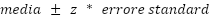
\includegraphics[width=5.55208in,height=3.65625in]{media/image1.png}

\textbf{esempio}
\end{quote}

\begin{itemize}
\item
  Preemptive: quando arriva un nuovo processo con CPU burst minore del
  CPU burst rimanente per il processo correntemente in esecuzione, il
  nuovo processo prende la CPU.
\end{itemize}

\begin{quote}
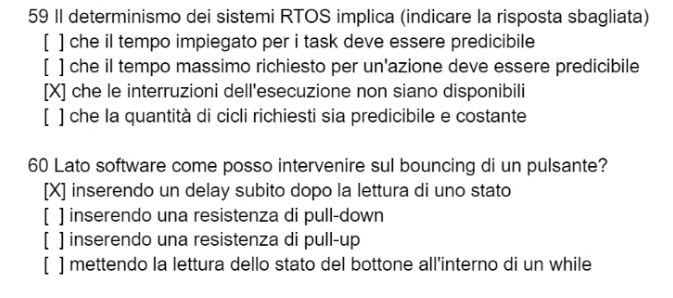
\includegraphics[width=5.70833in,height=3.63542in]{media/image21.png}

\textbf{esempio}
\end{quote}

Priority scheduling

Si usa un valore numerico per indicare quale processo fare prima, più il
valore è alto più velocemente deve accedere alla CPU; più il tempo di
attesa in coda aumenta per un processo più il valore della sua priorità
aumenta (aging).

Round Robin

Unico algoritmo visto fino ad ora adatto ai S.O. time sharing, è una
variante del FCFS.

Utilizza uno scheduler chiamato Round Robin dove la coda è gestita in
maniera circolare, dove ogni volta che un processo viene messo in
esecuzione, lo scheduler imposta un timer che ne limita il tempo di
esecuzione.

Code multiple

Questo algoritmo gestisce i processi di classe diverse; divisi in
foreground, quelli interattivi, e background (quelli batch).

In questo algoritmo la ready queue viene partizionata in più code
separate e ciascun processo è associato in modo statico ad una coda.

La particolarità è l'utilizzo di scheduler diversi per cose diverse, ad
esempio RR sui processi foreground e FCFS per i processi in background.

Per sapere da che coda prelevo il prossimo processo da eseguire si
utilizzano scheduling tra le code che possono essere:

\begin{itemize}
\item
  il non eseguire nessun processo della coda n se la coda n-1 non è
  vuota;
\item
  il definire dei quanti di tempo tra le code.
\end{itemize}

Code multiple con feedback

Nella code multiple normale ogni processo rimane sempre nella stessa
coda, si può invece fare in modo che i processi mutino dinamicamente
posizione, ad esempio in funzione del CPU burst che hanno.

Andando a creare un struttura dove la coda di livello più alto è quella
che contiene i processi con CPU burst inferiore.

Un processo viene inserito inizialmente nella coda più veloce per poi
retrocedere alla coda di livello inferiore quando non termina nel time
slice di quella coda.

\paragraph{CONCORRENZA}\label{concorrenza}

I processi possono essere eseguiti in modo:

\begin{itemize}
\item
  Concorrente: competono per l'accesso ad una risorsa;
\item
  Parallelo: sono eseguiti su diverse unità funzionali.
\end{itemize}

Qualunque sia l'esecuzione si generano problematiche
sull\textquotesingle integrità dei dati condivisi, con il \textbf{race
condition} si \emph{indica l'accesso a dati senza sincronizzazione e
controlli}; per ovviare al problema si utilizzano parti di codice dette
atomiche.

\subparagraph{\texorpdfstring{\emph{Critical
section}}{Critical section}}\label{critical-section}

È una parte di codice, costruita attorno alle variabili condivise, che
avranno un unico utilizzatore andando a scongiurare l'inconsistenza.

\emph{Una Sezione Critica (CS) è una porzione di codice in cui i dati
condivisi da processi cooperanti possono essere manipolati}

La CS è preceduta da una sezione di ingresso e una di uscita.

Ogni thread ha una critical section in cui accedere per modificare
variabili condivise, l\textquotesingle esecuzione di queste parti deve
garantire il MUTEX (mutua esclusione, è un meccanismo di blocco).

Il Thread non deve rimanere bloccato per sempre (Liveness), per questo
tramite il Bounded waiting, al thread può essere bloccato l'accesso solo
un numero limitato di volte.

\subparagraph{\texorpdfstring{\emph{Test and
Set}}{Test and Set}}\label{test-and-set}

In questa modalità si utilizzano variabili do lock, allocate all'interno
della memoria condivisa che funziona come lucchetto; se per esempio
questa cella ha valore 0 allora è possibile accedere alla variabile
altrimenti no.

Il valore viene settato dal processo che utilizza la risorsa nella CS.

Un problema di questa modalità è l'interruzione forzata tramite
interrupt dei processi che aspettano la variabile in lock; per ovviare è
stato creato il Test and Set Lock (TSL) una variabile che effettua i
controlli.

\subparagraph{\texorpdfstring{\emph{Semafori}}{Semafori}}\label{semafori}

Per superare l'impossibilità della generalizzazione delle regioni
critiche (difficoltà nel risolvere problemi complessi) sono nati i
semafori.

Un semaforo ``S'' è una variabile intera cui si può accedere, escludendo
l'inizializzazione, solo tramite due operazioni atomiche predefinite:
wait() e signal().

Al contrario del MUTEX, dove un processo deve detenere il mutex prima di
poter acquisire la risorsa, un semaforo è un meccanismo di segnalazione
dove i processi possono indicare se stanno acquisendo o rilasciando la
risorsa.

Quindi ricapitolando:

\begin{itemize}
\item
  I mutex hanno lo scopo di proteggere una risorsa condivisa, in modo
  che più processi non possano accedervi contemporaneamente;
\item
  un semaforo è un meccanismo di segnalazione tra processi e serve a
  condividere una risorsa che può essere usata contemporaneamente da un
  numero limitato di processi
\end{itemize}

\subparagraph{\texorpdfstring{\emph{Problemi
concorrenza}}{Problemi concorrenza}}\label{problemi-concorrenza}

Quando più processi concorrono per una risorsa e si applicano algoritmi
per gestirli si può incappare in alcuni errori:

\begin{itemize}
\item
  Busy waiting: si verifica quando un thread attende il verificarsi di
  una condizione (come la modifica di un semaforo) e lo fa verificando
  continuamente se la condizione sia diventata vera. Questo consuma
  tempo in CPU;
\item
  Starvation: avviene se un thread in attesa di una certa risorsa, non
  riesce mai ad accedervi perché arrivano continue richieste da thread
  con privilegi maggiori;
\item
  Deadlock: due o più thread aspettano indefinitamente un evento che può
  essere causato solo da uno dei thread bloccati;
\item
  Producer \& Consumer: due processi condividono un buffer di dimensione
  limitata, il ``produttore'' riempie un buffer, un item alla volta,
  finchè non è pieno e il ``consumatore'' svuota il buffer, un item alla
  volta finchè non è vuoto;
\item
  Readers \& Writers: thread scrittori e lettori devono accedere in modo
  concorrente ad un file, dove più letture possono avvenire
  contemporaneamente ma le scritture sono esclusive;
\item
  5 filosofi: in questo problema si usa un esempio dove ci sono 5 (o n,
  dove n\textgreater1) filosofi, che rappresentano i processi, a tavola
  per mangiare e pensare. Se un filosofo vuole mangiare deve usare due
  bastoncini ma tra un filosofo e l'altro c'e' un bastoncino solo, ogni
  filosofo può prendere solo una bacchetta alla volta e non può
  sottrarre bacchette dalle mani degli altri filosofi.
\end{itemize}

\begin{quote}
In questo esempio è impossibile che tutti i filosofi mangino allo stesso
tempo altrimenti si ruberebbero le risorse fra loro, per questo in
maniera alternata i filosofi devono mangiare e pensare.
\end{quote}

\subparagraph{\texorpdfstring{\emph{Monitor}}{Monitor}}\label{monitor}

I monitor sono costrutti di livello più alto rispetto ai semafori, ogni
monitor è una struttura dati (o un oggetto) che permette la mutua
esclusione e la sincronizzazione su strutture dati condivise da più
thread ed un solo thread alla volta può essere attivo all'interno di un
monitor.

Il monitor:

\begin{itemize}
\item
  garantisce la mutua esclusione (un solo thread alla volta può eseguire
  il codice contenuto nel monitor);
\item
  la possibilità di usare metodi pubblici utilizzabili da processi;
\item
  un insieme di variabili di condizione su cui possono essere invocate
  le primitive wait e signal.
\end{itemize}

L'ipotesi fondamentale per la realizzazione di semafori e monitor è
l'esistenza di memoria condivisa a cui i diversi thread possono fare
riferimento; sfortunatamente nei S.O. moderni non esiste shared memory.

Per ovviare al problema si utilizzano tecniche di message passing.

\paragraph{GESTIONE DELLA MEMORIA}\label{gestione-della-memoria}

Per funzionare c'è bisogno di due tipi di indirizzi che sono fra loro
uniti tramite un legame, questi indirizzi sono:

\begin{itemize}
\item
  Indirizzo fisico: è l\textquotesingle indirizzo nello spazio di
  memoria centrale che individua in modo univoco una parola in esso
  contenuta;
\item
  Indirizzo logico: è astratto ed esiste solo
  all\textquotesingle interno dello spazio di indirizzamento del
  processo, e ne rappresenta lo spiazzamento rispetto alla prima parola.
  \hl{Questo indirizzo viene utilizzato come riferimento per accedere
  alla posizione di memoria fisica}.
\end{itemize}

La corrispondenza fra i due indirizzi può avvenire durante la
compilazione, durante il caricamento o in esecuzione.

\subparagraph{\texorpdfstring{\emph{Rilocazione}}{Rilocazione}}\label{rilocazione}

È quando un programma viene allocato in memoria, quindi in questo
momento si decide l'indirizzo fisico che avrà.

La rilocazione avviene in maniera:

\begin{itemize}
\item
  Statica: nel momento di esecuzione il S.O., tramite il LOADER, decide
  lo spazio di memoria dove andrà allocato il processo.
\item
  Dinamica: il programma viene caricato in memoria ogni esecuzione,
  andando a cambiare indirizzo.
\end{itemize}

\subparagraph{\texorpdfstring{\emph{MMU}}{MMU}}\label{mmu}

Detto anche MEMORY-MANAGEMENT UNIT è un dispositivo con il compito di
eseguire la corrispondenza tra indirizzi in fase di esecuzione. Ciò è
possibile grazie al registro di rilocazione, dove la somma fra questo
valore e la parte indirizzo della istruzione (indirizzo logico) crea
l'indirizzo fisico.

\subparagraph{\texorpdfstring{\emph{Politiche di
allocazione}}{Politiche di allocazione}}\label{politiche-di-allocazione}

Insieme di regole per gestire la memoria, le politiche vengono valutate
tramite:

\begin{enumerate}
\def\labelenumi{\arabic{enumi}.}
\item
  Memoria sprecata;
\item
  Sovraccarico temporale: complessità computazionale delle operazioni di
  allocazione/deallocazione;
\item
  Sovraccarico nelle operazioni di accesso alla memoria
\end{enumerate}

Le allocazioni possono essere:

\begin{itemize}
\item
  \textbf{Contigue}: i programmi salvati vengono messi uno dopo l'altro
  in base all'avvio, ne esistono 4 tipologie:
\end{itemize}

\begin{enumerate}
\def\labelenumi{\arabic{enumi}.}
\item
  \emph{Monitor Monoprocesso}: modo più semplice, la memoria viene
  divisa in due dove in una area viene allocata la parte residente del
  S.O. e nell'altra vengono allocati i processi transienti.
\item
  \emph{Statica}: suddividiamo la memoria in modo che in ogni partizione
  (di dimensione fissa) si possa caricare un programma e quindi fare
  eseguire un processo. Si usa il TDP, una tabella di descrizione delle
  partizioni, per monitorare lo stato delle partizioni.
\item
  \emph{Dinamica}: La suddivisione della memoria avviene dinamicamente
  in base alle esigenze dei processi, quindi non c'è il problema di non
  avere partizioni troppo piccole per alcuni processi; anche qui
  necessito del TDP in unione con una lista delle aree libere in
  memoria. Con la partizione dinamica abbiamo il problema della
  frammentazione esterna infatti si possono creare delle aree libere tra
  le partizioni che non possono essere utilizzate.
\item
  \emph{Segmentazione}: creata per superare la frammentazione esterna,
  andando a ridurre le dimensioni delle zone allocate andando a dividere
  un programma in \ul{segmenti} che verrà allocato in modo contiguo.
\end{enumerate}

\begin{itemize}
\item
  \textbf{NON contigue}: si basa sulla suddivisione del processo in
  pagine logiche con corrispondenti pagine fisiche. Sostanzialmente
  viene allocata solo la parte di programma utilizzato.
\end{itemize}

\begin{quote}
Questa tecnica è detta paging o paginazione, colui che si occupa di
caricare (\emph{swap-in}) o deallocare (\emph{swap-out}) è detto pager,
se al caricamento di una pagina il componente non la trova in memoria o
c'è un errore nella gestione degli indirizzi viene generato un page
fault.

Quando avviene l'errore, dovuto alla mancanza della pagina, si genera un
segnale di \emph{trap} che informa il S.O, a questo punto il S.O. cerca
nel disco la pagina mancante e la carica nella memoria fisica; al
caricamento si modifica una tabella che ogni processo ha che indica
quali pagine contiene.

È cruciale scegliere bene il meccanismo di sostituzione delle pagine in
modo da tenere basso il numero dei page fault.
\end{quote}

\subparagraph{\texorpdfstring{\emph{Algoritmi di
caricamento}}{Algoritmi di caricamento}}\label{algoritmi-di-caricamento}

I diversi approcci alla scelta della pagina da scaricare sono:

\begin{enumerate}
\def\labelenumi{\arabic{enumi}.}
\item
  FIFO: l'algoritmo associa ad ogni pagina il tempo in cui è stata
  caricata in memoria e, se c'è necessità di scaricare una pagina,
  sceglie la pagina più vecchia;
\item
  Least Recently Used (LRU): l'algoritmo associa a ciascuna pagina
  l\textquotesingle istante in cui è stata usata per
  l\textquotesingle ultima volta e in caso di page fault con swap
  scarica la pagina che non viene acceduta da più tempo;
\item
  Least Frequently Used (LFU): viene usato un contatore che mantiene il
  numero degli accessi e viene scaricata la pagina che ha avuto in
  numero minore di hit;
\item
  Most Frequently Used (MFU): viene usato un contatore che mantiene il
  numero degli accessi e si scarica la pagina che ha avuto in numero
  maggiore di hit;
\end{enumerate}

\paragraph{GESTIONE DEI FILE SYSTEM}\label{gestione-dei-file-system}

Il file system è la parte del SO che si occupa di mantenere i
dati/programmi in modo persistente tramite file e directory.

\subparagraph{Accesso ai file}\label{accesso-ai-file}

In questo tipo di accesso i byte possono essere letti in qualsiasi
ordine, nei moderni sistemi operativi tutti i file sono automaticamente
ad accesso diretto.

I file system esistenti sono tutti di tipo gerarchico è utilizzano i
path name per indicare la posizione univoca di ogni file.

Si utilizza un grafo ad albero per determinare le posizioni, con la
radice principale detta ``root directory''; ogni file è univocamente
determinato dal cammino che lo collega alla radice.

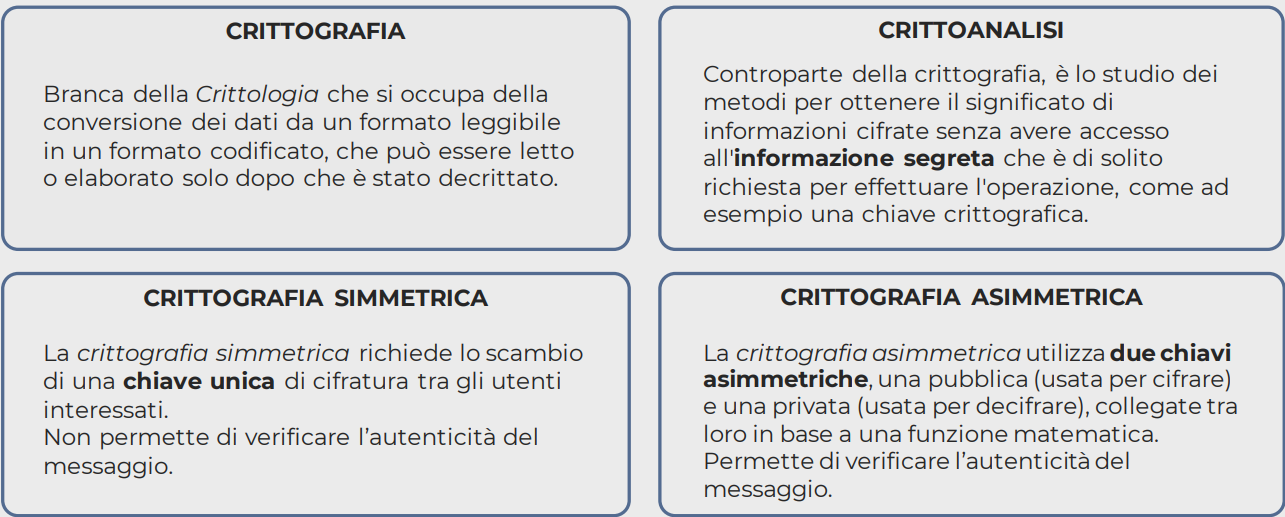
\includegraphics[width=5.82292in,height=3.875in]{media/image20.png}

\subparagraph{Implementazione FS}\label{implementazione-fs}

Per creare un nostro FS dobbiamo risolvere 3 quesiti:

\begin{enumerate}
\def\labelenumi{\arabic{enumi}.}
\item
  \textbf{Implementazione file}: normalmente i dati sono memorizzati in
  unità di ampiezza fissa e si devono memorizzare gli attributi e la
  posizione dei singoli blocchi;
\item
  \textbf{Implementazione directory}: le cartelle sono file con uno
  specifico formato;
\item
  \textbf{Gestione disco}: per farlo dobbiamo tenere traccia della root
  directory e anche in quali spazi del disco ci sono file e dove no.
\end{enumerate}

Implementazione file

Per allocare i file si può utilizzare la tecnica dell'allocazione
contigua che consiste nel memorizzare ogni file o in un gruppo di
blocchi contigui detti \emph{run}.

Questo porta enormi svantaggi come la possibilità di sprecare spazio se
l'ultimo blocco non è del tutto pieno e nel disco saranno presenti buchi
non grandi abbastanza per tenere altri file nelle parti di file
cancellate.

\emph{Esempio:}

File allocati in maniera
contigua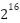
\includegraphics[width=6.26772in,height=0.375in]{media/image3.png}

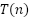
\includegraphics[width=2.16667in,height=0.5625in]{media/image5.png}

Caso di file più piccolo rispetto ai blocchi

Disco dopo la cancellazione di alcune
parti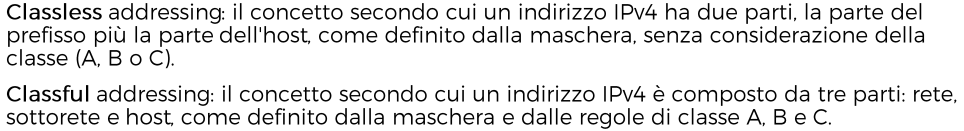
\includegraphics[width=6.26772in,height=0.375in]{media/image6.png}

Un'altra tecnica è quella delle liste concatenate, dove ogni blocco
contiene l'indirizzo di quello successivo, in questo modo non c'è
frammentazione esterna e il file può essere salvato su più parti di
memoria portando però ad un'accesso alle informazioni molto lento.

La tecnica principale usata da Unix è la \emph{Index-node} o
\emph{i-node}, in questo modo solo gli i-node dei file in uso devono
risiedere in RAM e lo spazio è proporzionale al numero massimo di file
aperti e non dipende dall'ampiezza del disco.

Infatti ogni \hl{\emph{i-node} ha associato un numero univoco
all\textquotesingle interno del dispositivo e ogni file presente è
identificato come un
\href{https://it.wikipedia.org/wiki/Collegamento_fisico}{collegamento
fisico} all\textquotesingle i-node tramite il suo numero. Quando un
programma cerca di accedere ad un file tramite un nome (es.
documento.txt), il
\href{https://it.wikipedia.org/wiki/Sistema_operativo}{sistema
operativo} cerca l\textquotesingle i-node corrispondente e recupera
tutte le informazioni sopra descritte per operare correttamente con il
file.}

Implementazione Directory

Devono permettere di recuperare tutte le informazioni relative ai file
contenuti il punto fondamentale è associare il nome del file ad
attributi e dati (indirizzo/i dei blocchi).

La soluzione più semplice è far contenere alla directory una tabella con
un elemento per ogni file, dove attributi e indirizzi dei blocchi del
file X sono memorizzati direttamente nell'elemento della tabella
relativo ad X (usata da FAT).

Gestione disco

Tutti i FS dividono i file in blocchi NON CONTIGUI di ampiezza fissata
ed eseguono letture e scritture su blocchi o multipli.

Per decidere l'ampiezza dei blocchi dobbiamo chiederci che
caratteristica vogliamo per il nostro FS, con blocchi piccoli usiamo
meglio lo spazio disco (diminuiscono la frammentazione interna) con
blocchi grandi velocizziamo gli accessi.

Per tenere traccia dei blocchi liberi su disco abbiamo 2 alternative:

\begin{enumerate}
\def\labelenumi{\arabic{enumi}.}
\item
  Free list: lista concatenata di blocchi pieni di indirizzi di blocchi
  liberi;
\item
  Bitmap: una mappa di bit con un bit per ogni blocco, mantiene la
  contiguità dei blocchi.
\end{enumerate}

\emph{Esempio}:

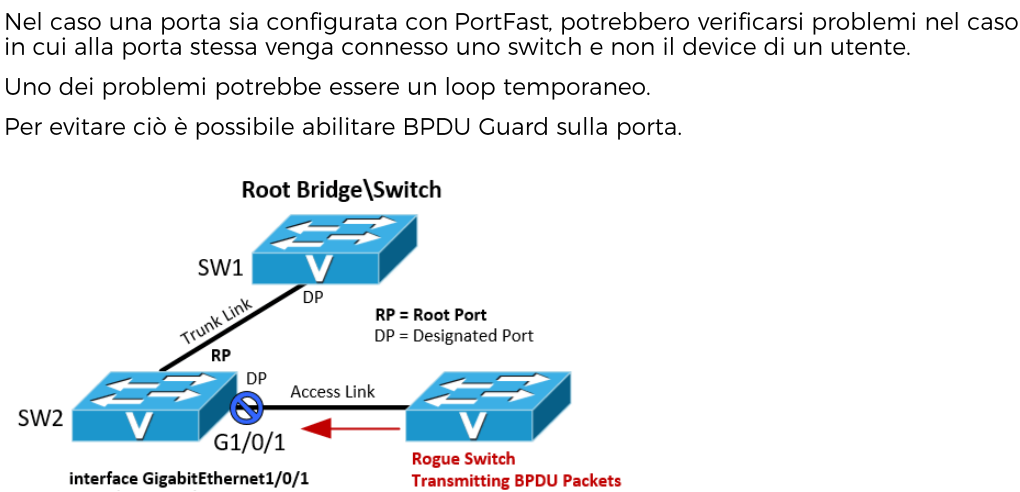
\includegraphics[width=5.65228in,height=4.14063in]{media/image15.png}

Gestione errori e affidabilità

Se una traccia ha un settore difettoso il FS in automatico sostituisce
il settore difettoso con uno di riserva, andando a slittare tutto per
evitare il problema.

Il FS esegue backup periodici in caso di crash e problemi accidentali in
modo da non perdere dati.

Con \emph{Stable Storage} si indica una tecnica che permette di mettersi
al riparo da errori che si verificano durante una scrittura, infatti
nello stable storage, ogni volta che eseguiamo una write si garantisce
che il valore scritto è corretto oppure è uguale a quello vecchio.

\paragraph{GESTIONE DISPOSITIVI I/O}\label{gestione-dispositivi-io}

I dispositivi I/O sono molti ed eterogenei con obiettivi differenti
(memorizzazione, trasmissione, interazione, ecc) per questo è necessario
uniformare gli standard per alleggerire la loro gestione da parte del
S.O.

Il kernel ha un sottosistema apposito per la gestione I/O con driver che
offrono un\textquotesingle interfaccia uniforme per l'accesso ai
dispositivi.

Alcuni meccanismi hardware sono comuni fra tutti i dispositivi, e sono:

\begin{itemize}
\item
  Porta: punto di connessione fisica (via cavo o etere) tra il sistema
  di calcolo e il device di I/O;
\item
  Bus: insieme di connessioni al sistema di calcolo utilizzate da più
  dispositivi contemporaneamente;
\item
  Controller: processore dedicato con microcodice che svolge attività
  specializzate sul device di I/O.
\end{itemize}

\subparagraph{Registri e controller}\label{registri-e-controller}

Tipicamente una porta di I/O opera sulla base di 4 registri:

\begin{enumerate}
\def\labelenumi{\arabic{enumi}.}
\item
  Status: bit che indicano lo stato della porta ;
\item
  Control: viene usato per attivare un comando o per cambiare il modo
  operativo del dispositivo;
\item
  Data-in: byte disponibili in lettura;
\item
  Data-out: byte disponibili in scrittura.
\end{enumerate}

Per accedere ai registri si usa il controller e l'accesso può avvenire:

\begin{itemize}
\item
  Mappando i dispositivi in memoria: i registri sono visti nello spazio
  di indirizzamento della memoria, ciò permette di scrivere driver in
  linguaggio ad alto livello andando a sacrificare la protezione;
\item
  Mappando i dispositivi sull' I/O: si accede ai registri tramite
  istruzioni specifiche evitando problemi di gestione cache.
\end{itemize}

Comunicazione controller

Per comunicare con il controller possiamo usare diversi modi:

\begin{itemize}
\item
  \textbf{Polling}: la CPU controlla periodicamente lo stato del
  controller per verificare se una operazione è completata o no.
\end{itemize}

\begin{quote}
Si basa sul paradigma handshaking con l'utilizzo di 2 bit per coordinare
la relazione produttore/consumatore (il 1° detto bit busy, il 2° command
ready); chi controlla il bit busy è in polling.

Questo procedimento diventa inefficiente perchè, sebbene le
interrogazioni siano frequenti, si trova raramente un dispositivo
libero;
\end{quote}

\begin{itemize}
\item
  \textbf{Interrupt}: il controller segnala alla CPU il completamento
  dell'operazione richiesta, infatti è presente un hardware apposito, la
  linea di richiesta dell'interrupt, controllato direttamente dalla CPU.
\end{itemize}

\begin{quote}
Quando si rileva un segnale la CPU blocca quello che sta facendo ed
esegue una routine apposita detta \emph{interrupt handler}, il compito
della routine è quello di determinare perché la CPU si è bloccata e
portare a termine l'operazione I/O;
\end{quote}

\begin{itemize}
\item
  \textbf{DMA} (Direct Memory Access): la segnalazione alla CPU viene
  mandata per blocchi e non per byte, grazie ad un accesso diretto del
  controller DMA sulla memoria centrale. Inoltre la CPU interviene
  direttamente nella gestione degli interrupt e questa attività è molto
  dispersiva, per questo può essere utile un controller dedicato che
  trasferisca i dati direttamente dall'I/O alla memoria centrale senza
  contattare la CPU.
\end{itemize}

\begin{quote}
Il nuovo controller DMA trasferisce su 2 livelli:
\end{quote}

\begin{enumerate}
\def\labelenumi{\arabic{enumi}.}
\item
  \textbf{CPU-DMA}: la CPU chiede al controller DMA di avviare il
  trasferimento e il controller DMA segnala il completamento (tramite
  interrupt);
\item
  \textbf{DMA-Device Controller-Memoria}: il controller DMA agisce
  trasferendo i dati dalla memoria centrale al controller del device e
  viceversa.
\end{enumerate}

\subparagraph{Interfacce per applicazioni
{[}Driver{]}}\label{interfacce-per-applicazioni-driver}

Il S.O. deve offrire alle applicazioni un\textquotesingle interfaccia
astratta per far utilizzare il sistema I/O alle applicazioni, per farlo
si necessita dei driver.

I driver costituiscono dunque lo strato del S.O. più vicino all'hardware
dell'I/O. È un software, spesso scritto in assembly, che permette ad un
sistema operativo di pilotare un dispositivo hardware.

In questo modo il S.O. agisce in modo indipendente dall'hardware e
questo va a vantaggio di chi implementa il S.O. e di chi produce
hardware.

\subparagraph{Sottosistema I/O -
Servizi}\label{sottosistema-io---servizi}

I principali servizi offerti dal sottosistema di I/O del kernel sono:

\begin{itemize}
\item
  \textbf{Scheduling}: cioè gestire l'ordine con cui le richieste di I/O
  sono gestite, il problema è particolarmente rilevante nella gestione
  degli accessi al disco;
\item
  \textbf{Buffering}: si utilizza un buffer, cioè una regione di memoria
  che contiene dati mentre questi sono trasferiti da un dispositivo, per
  permettere la bufferizzazione. La tecnica è essenziale perché i
  dispositivi potrebbero avere velocità diverse oppure avere diverse
  dimensioni dei blocchi trasferiti. Un'altra importante caratteristica
  è la semantica di copia, cioè garantire che la versione dei dati
  scritta su un dispositivo sia la stessa versione presente in memoria;
\item
  \textbf{Caching}. si utilizza una cache per migliorare le prestazioni
  dei dispositivi di I/O, al contrario del buffer la cache non può
  contenere dati di cui non esiste altra copia;
\item
  \textbf{Spooling}: si utilizza lo spool, cioè un buffer contenente
  output per dispositivi che non possono accettare flussi di dati da più
  processi contemporaneamente, come ad esempio la stampante.
\end{itemize}

\begin{quote}
Lo spooler è l\textquotesingle unico programma che ha accesso diretto
alla periferica, e gestisce il buffer offrendo agli utenti alcune
operazioni aggiuntive come la visualizzazione della coda di attesa dei
processi o la cancellazione/sospensione di uno di essi.
\end{quote}
